\PassOptionsToPackage{unicode=true}{hyperref} % options for packages loaded elsewhere
\PassOptionsToPackage{hyphens}{url}
%
\documentclass[10pt,xcolor=table,color={dvipsnames,usenames},ignorenonframetext,usepdftitle=false,french,aspectratio=169]{beamer}
\setbeamertemplate{caption}[numbered]
\setbeamertemplate{caption label separator}{: }
\setbeamercolor{caption name}{fg=normal text.fg}
\beamertemplatenavigationsymbolsempty
\usepackage{caption}
\captionsetup{skip=0pt,belowskip=0pt}
%\setlength\abovecaptionskip{-15pt}
\usepackage{lmodern}
\usepackage{amssymb,amsmath,mathtools,multirow}
\usepackage{float,hhline}
\usepackage{tikz}
\usepackage{mathtools}
\usepackage{ifxetex,ifluatex}
\usepackage{fixltx2e} % provides \textsubscript
\ifnum 0\ifxetex 1\fi\ifluatex 1\fi=0 % if pdftex
  \usepackage[T1]{fontenc}
  \usepackage[utf8]{inputenc}
  \usepackage{textcomp} % provides euro and other symbols
\else % if luatex or xelatex
  \usepackage{unicode-math}
  \defaultfontfeatures{Ligatures=TeX,Scale=MatchLowercase}
\fi
\usetheme[coding=utf8,language=english,
,titlepagelogo=img/SACElogo
]{TorinoTh}
% use upquote if available, for straight quotes in verbatim environments
\IfFileExists{upquote.sty}{\usepackage{upquote}}{}
% use microtype if available
\IfFileExists{microtype.sty}{%
\usepackage[]{microtype}
\UseMicrotypeSet[protrusion]{basicmath} % disable protrusion for tt fonts
}{}
\IfFileExists{parskip.sty}{%
\usepackage{parskip}
}{% else
\setlength{\parindent}{0pt}
\setlength{\parskip}{6pt plus 2pt minus 1pt}
}
\usepackage{hyperref}
\hypersetup{
            pdfauthor={Anna Smyk and Tanguy Barthelemy},
            pdfborder={0 0 0},
            breaklinks=true}
\urlstyle{same}  % don't use monospace font for urls
\newif\ifbibliography
\newlength{\cslhangindent}
\setlength{\cslhangindent}{1.5em}
\newlength{\csllabelwidth}
\setlength{\csllabelwidth}{3em}
\newenvironment{CSLReferences}[2] % #1 hanging-ident, #2 entry spacing
 {% don't indent paragraphs
  \setlength{\parindent}{0pt}
  % turn on hanging indent if param 1 is 1
  \ifodd #1 \everypar{\setlength{\hangindent}{\cslhangindent}}\ignorespaces\fi
  % set entry spacing
  \ifnum #2 > 0
  \setlength{\parskip}{#2\baselineskip}
  \fi
 }%
 {}
\usepackage{color}
\usepackage{fancyvrb}
\newcommand{\VerbBar}{|}
\newcommand{\VERB}{\Verb[commandchars=\\\{\}]}
\DefineVerbatimEnvironment{Highlighting}{Verbatim}{commandchars=\\\{\}}
% Add ',fontsize=\small' for more characters per line
\usepackage{framed}
\definecolor{shadecolor}{RGB}{248,248,248}
\newenvironment{Shaded}{\begin{snugshade}}{\end{snugshade}}
\newcommand{\AlertTok}[1]{\textcolor[rgb]{0.94,0.16,0.16}{#1}}
\newcommand{\AnnotationTok}[1]{\textcolor[rgb]{0.56,0.35,0.01}{\textbf{\textit{#1}}}}
\newcommand{\AttributeTok}[1]{\textcolor[rgb]{0.77,0.63,0.00}{#1}}
\newcommand{\BaseNTok}[1]{\textcolor[rgb]{0.00,0.00,0.81}{#1}}
\newcommand{\BuiltInTok}[1]{#1}
\newcommand{\CharTok}[1]{\textcolor[rgb]{0.31,0.60,0.02}{#1}}
\newcommand{\CommentTok}[1]{\textcolor[rgb]{0.56,0.35,0.01}{\textit{#1}}}
\newcommand{\CommentVarTok}[1]{\textcolor[rgb]{0.56,0.35,0.01}{\textbf{\textit{#1}}}}
\newcommand{\ConstantTok}[1]{\textcolor[rgb]{0.00,0.00,0.00}{#1}}
\newcommand{\ControlFlowTok}[1]{\textcolor[rgb]{0.13,0.29,0.53}{\textbf{#1}}}
\newcommand{\DataTypeTok}[1]{\textcolor[rgb]{0.13,0.29,0.53}{#1}}
\newcommand{\DecValTok}[1]{\textcolor[rgb]{0.00,0.00,0.81}{#1}}
\newcommand{\DocumentationTok}[1]{\textcolor[rgb]{0.56,0.35,0.01}{\textbf{\textit{#1}}}}
\newcommand{\ErrorTok}[1]{\textcolor[rgb]{0.64,0.00,0.00}{\textbf{#1}}}
\newcommand{\ExtensionTok}[1]{#1}
\newcommand{\FloatTok}[1]{\textcolor[rgb]{0.00,0.00,0.81}{#1}}
\newcommand{\FunctionTok}[1]{\textcolor[rgb]{0.00,0.00,0.00}{#1}}
\newcommand{\ImportTok}[1]{#1}
\newcommand{\InformationTok}[1]{\textcolor[rgb]{0.56,0.35,0.01}{\textbf{\textit{#1}}}}
\newcommand{\KeywordTok}[1]{\textcolor[rgb]{0.13,0.29,0.53}{\textbf{#1}}}
\newcommand{\NormalTok}[1]{#1}
\newcommand{\OperatorTok}[1]{\textcolor[rgb]{0.81,0.36,0.00}{\textbf{#1}}}
\newcommand{\OtherTok}[1]{\textcolor[rgb]{0.56,0.35,0.01}{#1}}
\newcommand{\PreprocessorTok}[1]{\textcolor[rgb]{0.56,0.35,0.01}{\textit{#1}}}
\newcommand{\RegionMarkerTok}[1]{#1}
\newcommand{\SpecialCharTok}[1]{\textcolor[rgb]{0.00,0.00,0.00}{#1}}
\newcommand{\SpecialStringTok}[1]{\textcolor[rgb]{0.31,0.60,0.02}{#1}}
\newcommand{\StringTok}[1]{\textcolor[rgb]{0.31,0.60,0.02}{#1}}
\newcommand{\VariableTok}[1]{\textcolor[rgb]{0.00,0.00,0.00}{#1}}
\newcommand{\VerbatimStringTok}[1]{\textcolor[rgb]{0.31,0.60,0.02}{#1}}
\newcommand{\WarningTok}[1]{\textcolor[rgb]{0.56,0.35,0.01}{\textbf{\textit{#1}}}}
\usepackage{graphicx,grffile}
\makeatletter
\def\maxwidth{\ifdim\Gin@nat@width>\linewidth\linewidth\else\Gin@nat@width\fi}
\def\maxheight{\ifdim\Gin@nat@height>\textheight\textheight\else\Gin@nat@height\fi}
\makeatother
% Scale images if necessary, so that they will not overflow the page
% margins by default, and it is still possible to overwrite the defaults
% using explicit options in \includegraphics[width, height, ...]{}
\setkeys{Gin}{width=\maxwidth,height=\maxheight,keepaspectratio}
% Prevent slide breaks in the middle of a paragraph:
\widowpenalties 1 10000
\raggedbottom
\AtBeginPart{
  \let\insertpartnumber\relax
  \let\partname\relax
  \frame{\partpage}
}
\AtBeginSection{
  \ifbibliography
  \else
    \begin{frame}[noframenumbering]{Contents}
    \tableofcontents[currentsection, hideothersubsections]
    \end{frame}
  \fi
}
\setlength{\emergencystretch}{3em}  % prevent overfull lines
\providecommand{\tightlist}{%
  %\setlength{\itemsep}{0pt}
  \setlength{\parskip}{0pt}
  }
\setcounter{secnumdepth}{0}

% set default figure placement to htbp
\makeatletter
\def\fps@figure{htbp}
\makeatother

\usepackage{dsfont}
\usepackage{stmaryrd}
\usepackage[normalem]{ulem}
\usepackage{fontawesome5}
\usepackage{tikz,pgfplots}
\pgfplotsset{compat=1.17}
\pgfplotsset{samples=100}
\usepackage{animate}
 \usepackage{booktabs}

\usepackage{colortbl}

\DeclareMathOperator{\Cov}{Cov}
\newcommand{\cov}[2]{\Cov\left( #1\,,\,#2 \right)}

\DeclareMathOperator{\e}{e}
\renewcommand{\P}{\mathds{P}} %Apparement \P existe déjà ?
\newcommand\N{\mathds{N}}
\newcommand\R{\mathds{R}}


\newcommand\1{\mathds{1}}
\newcommand{\E}[2][]{{\mathds{E}}_{#1}
  \def\temp{#2}\ifx\temp\empty
  \else
    \left[#2\right]
  \fi
}
\newcommand{\V}[2][]{{\mathds{V}}_{#1}
  \def\temp{#2}\ifx\temp\empty
  \else
    \left[#2\right]
  \fi
}
\newcommand\ud{\,\mathrm{d}}


% blocks
\usepackage{environ}
\usepackage[tikz]{bclogo}

\tikzstyle{titlestyle} =[draw=black!80,fill=black!20, text=black,
 right=10pt, rounded corners]
\mdfdefinestyle{symmaryboxstyle}{
	linecolor=black!80, backgroundcolor = black!5,
	skipabove=\baselineskip, innertopmargin=\baselineskip,
	innerbottommargin=\baselineskip,
	userdefinedwidth=\textwidth,
	middlelinewidth=1.2pt, roundcorner=5pt,
	skipabove={\dimexpr0.5\baselineskip+\topskip\relax},
	frametitleaboveskip=\dimexpr-\ht\strutbox\relax,
	innerlinewidth=0pt,
}
\NewEnviron{summary}{%
\begin{mdframed}[style=symmaryboxstyle]
\vspace{-0.5em}
\BODY
\end{mdframed}
}
\makeatletter
% Open `\noalign` and check for overlay specification:
\def\rowcolor{\noalign{\ifnum0=`}\fi\bmr@rowcolor}
\newcommand<>{\bmr@rowcolor}{%
    \alt#1%
        {\global\let\CT@do@color\CT@@do@color\@ifnextchar[\CT@rowa\CT@rowb}% Rest of original `\rowcolor`
        {\ifnum0=`{\fi}\@gooble@rowcolor}% End `\noalign` and gobble all arguments of `\rowcolor`.
}
% Gobble all normal arguments of `\rowcolor`:
\newcommand{\@gooble@rowcolor}[2][]{\@gooble@rowcolor@}
\newcommand{\@gooble@rowcolor@}[1][]{\@gooble@rowcolor@@}
\newcommand{\@gooble@rowcolor@@}[1][]{\ignorespaces}

\newcommand{\rowc}[1]{\only<#1>{\\\rowcolor{processblue!40}}}
%\newcommand{\rowc}[1]{{\rowcolor<#1>{processblue!30}}
\newcommand{\cellc}[1]{\only<#1>{\cellcolor{processblue!40}}}
\newcommand{\supsp}[1]{\visible<#1>{\\}}

\title{Using JDemetra+ in R: from version 2 to version 3\\
Presentation 2: Seasonal adjustment in R}
\ateneo{TSACE Webinar, Wednesday December 14th 2022}
\author{Anna Smyk and Tanguy Barthelemy}
\date{}


\setrellabel{}

\setcandidatelabel{}

\rel{}
\division{With the collaboration of Alain Quartier-la-tente\\}

\departement{}
\makeatletter
\let\@@magyar@captionfix\relax
\makeatother


\begin{document}
\begin{frame}[plain,noframenumbering]
\titlepage
\end{frame}

\hypertarget{introduction}{%
\section{Introduction}\label{introduction}}

\begin{frame}{Seasonal adjustment: common steps}
\protect\hypertarget{seasonal-adjustment-common-steps}{}
\begin{itemize}
\tightlist
\item
  testing for seasonality (identify seasonal patterns for HF data)
\item
  pre-treatment
\item
  create customisezd variables for pre-treatment (e.g calendar
  regressors)
\item
  decomposition
\item
  retrieve output series
\item
  retrieve diagnostics
\item
  customize parameters
\item
  refresh data
\item
  \ldots{}
\item
  repeat..
\end{itemize}

This presentation will illustrate all this points, mainly in X13-Arima.
\end{frame}

\begin{frame}[fragile]{Context of use}
\protect\hypertarget{context-of-use}{}
Producing Seasonally adjusted series in R (with parameters customized
according to needs and previous diagnostics)

\begin{itemize}
\item
  not being aware of JD+ GUI existence
\item
  no workspace structure of data
\item
  time series objects in R
\item
  use exclusively JD+ algorithms and no other SA R packages (Seasonal,
  TBATS\ldots)
\end{itemize}

All the examples are related to ONE series. For an entire data set you
can of course use loops or \texttt{lapply()} type of functions
\end{frame}

\hypertarget{x13-and-some-tramo-seats}{%
\section{X13 (\ldots and some
Tramo-Seats)}\label{x13-and-some-tramo-seats}}

\hypertarget{quick-launch-with-default-specifications}{%
\subsection{Quick Launch with default
specifications}\label{quick-launch-with-default-specifications}}

\begin{frame}[fragile,allowframebreaks]{Running a Seasonal Adjustment
processing}
\protect\hypertarget{running-a-seasonal-adjustment-processing}{}
In version 2 \footnotesize

\begin{Shaded}
\begin{Highlighting}[]
\CommentTok{\# X13}
\NormalTok{sa\_x13\_v2 }\OtherTok{\textless{}{-}}\NormalTok{ RJDemetra}\SpecialCharTok{::}\FunctionTok{x13}\NormalTok{(y\_raw, }\AttributeTok{spec =} \StringTok{"RSA5c"}\NormalTok{)}
\CommentTok{\# see help pages for default spec names, identical in v2 and v3}
\CommentTok{\#Tramo{-}Seats}
\NormalTok{sa\_ts\_v2 }\OtherTok{\textless{}{-}}\NormalTok{ RJDemetra}\SpecialCharTok{::}\FunctionTok{tramoseats}\NormalTok{(y\_raw, }\AttributeTok{spec =} \StringTok{"RSAfull"}\NormalTok{)}
\end{Highlighting}
\end{Shaded}

In version 3 (printed model identical to v2) \footnotesize

\begin{Shaded}
\begin{Highlighting}[]
\CommentTok{\#X13}
\NormalTok{sa\_x13\_v3 }\OtherTok{\textless{}{-}}\NormalTok{ rjd3x13}\SpecialCharTok{::}\FunctionTok{x13}\NormalTok{(y\_raw, }\AttributeTok{spec =} \StringTok{"RSA5"}\NormalTok{)}
\NormalTok{sa\_x13\_v3}
\end{Highlighting}
\end{Shaded}

\begin{verbatim}
## RegARIMA
## Log-transformation: yes 
## SARIMA model:  (0,1,1) (0,1,1) 
## 
## Coefficients
##           Estimate Std. Error T-stat
## theta(1)  -0.72466    0.03740 -19.38
## btheta(1) -0.56372    0.04992 -11.29
## 
## Regression model:
##            Estimate Std. Error T-stat
## monday     0.016430   0.008647  1.900
## tuesday    0.012493   0.008603  1.452
## wednesday  0.006496   0.008621  0.754
## thursday  -0.003046   0.008598 -0.354
## friday     0.019581   0.008638  2.267
## saturday  -0.020445   0.008608 -2.375
## easter    -0.045446   0.017158 -2.649
## Number of observations:  354 
## Number of effective observations:  341 
## Number of parameters:  10 
## 
## Loglikelihood:  374.7681 
## Adjusted loglikelihood:  -1077.716 
## 
## Standard error of the regression (ML estimate):  0.07999264 
## AIC:  2175.432 
## AICC:  2176.099 
## BIC:  2213.751 
## 
## 
## Decomposition
## Monitoring and Quality Assessment Statistics: 
##     M stats
## m1    0.986
## m2    0.660
## m3    1.888
## m4    0.262
## m5    1.877
## m6    0.140
## m7    0.374
## m8    0.823
## m9    0.441
## m10   0.557
## m11   0.484
## q     0.799
## qm2   0.816
## 
## Final filters: 
## Seasonal filter:  
## Trend filter: 23 terms Henderson moving average
## 
## Diagnostics
## Relative contribution of the components to the stationary
## portion of the variance in the original series,
## after the removal of the long term trend (in %)
## 
##            Component
##  cycle        35.745
##  seasonal     49.917
##  irregular     6.601
##  calendar      2.726
##  others        0.000
##  total        94.989
## 
## Residual seasonality tests
##                 P.value
##  seas.ftest.i     0.977
##  seas.ftest.sa    0.992
##  seas.qstest.i    1.000
##  seas.qstest.sa   1.000
##  td.ftest.i       0.999
##  td.ftest.sa      0.999
## 
## 
## Final
## Last values
##             series       sa    trend seas       irr
## Jul 2018 108.12963 125.7729 112.5273    1 1.1177102
## Aug 2018  90.03625 116.6883 113.3824    1 1.0291574
## Sep 2018 116.46355 112.2071 113.8818    1 0.9852950
## Oct 2018 124.07923 109.5869 113.9926    1 0.9613510
## Nov 2018 136.04300 119.6826 113.7513    1 1.0521420
## Dec 2018 113.17850 124.2718 113.2503    1 1.0973202
## Jan 2019 108.28574 108.9028 112.6145    1 0.9670404
## Feb 2019 110.21151 114.3220 111.9838    1 1.0208800
## Mar 2019 122.43580 111.6401 111.4757    1 1.0014743
## Apr 2019 108.64593 108.2331 111.1456    1 0.9737949
## May 2019 111.25296 111.2931 110.9967    1 1.0026702
## Jun 2019 109.35264 105.3926 111.0227    1 0.9492889
\end{verbatim}

\begin{Shaded}
\begin{Highlighting}[]
\CommentTok{\#Tramo seats}
\NormalTok{sa\_ts\_v3 }\OtherTok{\textless{}{-}}\NormalTok{ rjd3tramoseats}\SpecialCharTok{::}\FunctionTok{tramoseats}\NormalTok{(y\_raw, }\AttributeTok{spec =} \StringTok{"RSAfull"}\NormalTok{)}
\end{Highlighting}
\end{Shaded}
\end{frame}

\begin{frame}[fragile]{Running only pre-adjustment}
\protect\hypertarget{running-only-pre-adjustment}{}
In version 2 \footnotesize

\begin{Shaded}
\begin{Highlighting}[]
\CommentTok{\# Reg{-}Arima part from X13 only (different default spec names, cf help pages)}
\NormalTok{regA\_v2 }\OtherTok{\textless{}{-}}\NormalTok{ RJDemetra}\SpecialCharTok{::}\FunctionTok{regarima\_x13}\NormalTok{(y\_raw, }\AttributeTok{spec =} \StringTok{"RG5c"}\NormalTok{)}

\CommentTok{\# Tramo only }
\NormalTok{tramo\_v2 }\OtherTok{\textless{}{-}}\NormalTok{ RJDemetra}\SpecialCharTok{::}\FunctionTok{regarima\_tramoseats}\NormalTok{(y\_raw,}\AttributeTok{spec =} \StringTok{"TRfull"}\NormalTok{)}
\end{Highlighting}
\end{Shaded}

In version 3 (not very different) \footnotesize

\begin{Shaded}
\begin{Highlighting}[]
\CommentTok{\#X13}
\NormalTok{sa\_regarima\_v3 }\OtherTok{\textless{}{-}}\NormalTok{ rjd3x13}\SpecialCharTok{::}\FunctionTok{regarima}\NormalTok{(y\_raw, }\AttributeTok{spec =} \StringTok{"RG5c"}\NormalTok{)}

\CommentTok{\#Tramo seats }
\CommentTok{\#sa\_tramo\_v3 \textless{}{-} rjd3tramoseats::tramo(y\_raw, spec = "TRfull")}

\CommentTok{\# "fast." versions...(just results, cf output structure)}
\end{Highlighting}
\end{Shaded}
\end{frame}

\begin{frame}[fragile]{Running only decomposition}
\protect\hypertarget{running-only-decomposition}{}
In version 2 \footnotesize

\begin{Shaded}
\begin{Highlighting}[]
\CommentTok{\# X11 (spec option)}
\NormalTok{X11\_v2 }\OtherTok{\textless{}{-}}\NormalTok{ RJDemetra}\SpecialCharTok{::}\FunctionTok{x13}\NormalTok{(y\_raw, }\AttributeTok{spec =} \StringTok{"X11"}\NormalTok{)}

\CommentTok{\#Tramo{-}Seats ? you }
\CommentTok{\#sa\_ts\_v2\textless{}{-}RJDemetra::tramoseats(y\_raw, spec = "RSAfull")}
\end{Highlighting}
\end{Shaded}

In version 3 \footnotesize

\begin{Shaded}
\begin{Highlighting}[]
\CommentTok{\#X11}
\NormalTok{x11\_v3 }\OtherTok{\textless{}{-}}\NormalTok{ rjd3x13}\SpecialCharTok{::}\FunctionTok{x11}\NormalTok{(y\_raw) }\CommentTok{\# specific function}
\CommentTok{\#Seats: you need an arima model}
\end{Highlighting}
\end{Shaded}
\end{frame}

\hypertarget{retrieving-output-and-data-visualization}{%
\subsection{Retrieving output and data
visualization}\label{retrieving-output-and-data-visualization}}

\begin{frame}[fragile]{``Model\_sa'' object structure in version 2
(1/2)}
\protect\hypertarget{model_sa-object-structure-in-version-2-12}{}
``Model\_sa'' is the resulting object of the estimation, it contains

\begin{itemize}
\tightlist
\item
  raw series\\
\item
  parameters (specification)\\
\item
  output series
\item
  diagnostics
\end{itemize}

All arranged in a specific way

\footnotesize

\begin{Shaded}
\begin{Highlighting}[]
\CommentTok{\# v2 "output"}
\NormalTok{Model\_sa }\OtherTok{\textless{}{-}}\NormalTok{ RJDemetra}\SpecialCharTok{::}\FunctionTok{x13}\NormalTok{(y\_raw, }\AttributeTok{spec =} \StringTok{"RSA5"}\NormalTok{)}

\NormalTok{Model\_sa}\SpecialCharTok{$}\NormalTok{regarima}
\NormalTok{Model\_sa}\SpecialCharTok{$}\NormalTok{decomposition}
\CommentTok{\#...}
\end{Highlighting}
\end{Shaded}
\end{frame}

\begin{frame}{``Model\_sa'' object structure in version 2}
\protect\hypertarget{model_sa-object-structure-in-version-2}{}
Organised by domain:

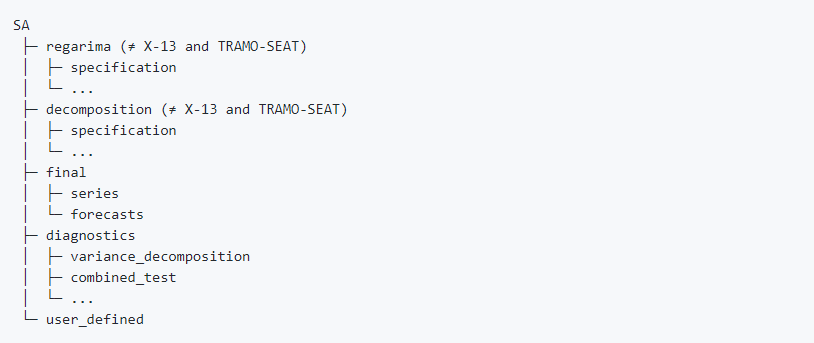
\includegraphics{img/sa_obj_struct.PNG} \{width=90\%\}
\end{frame}

\begin{frame}[fragile]{``Model\_sa'' object structure in version 3}
\protect\hypertarget{model_sa-object-structure-in-version-3}{}
Results vs specification\ldots and then by domain

\footnotesize

\begin{Shaded}
\begin{Highlighting}[]
\CommentTok{\# Model\_sa = sa\_x13\_v3}
\NormalTok{sa\_x13\_v3 }\OtherTok{\textless{}{-}}\NormalTok{ RJDemetra}\SpecialCharTok{::}\FunctionTok{x13}\NormalTok{(y\_raw, }\AttributeTok{spec =} \StringTok{"RSA5"}\NormalTok{)}
\NormalTok{sa\_x13\_v3}\SpecialCharTok{$}\NormalTok{result}
\NormalTok{sa\_x13\_v3}\SpecialCharTok{$}\NormalTok{estimation\_spec}
\NormalTok{sa\_x13\_v3}\SpecialCharTok{$}\NormalTok{result\_spec}
\NormalTok{sa\_x13\_v3}\SpecialCharTok{$}\NormalTok{user\_defined}
\end{Highlighting}
\end{Shaded}
\end{frame}

\begin{frame}{Differences from version 2 to version 3}
\protect\hypertarget{differences-from-version-2-to-version-3}{}
In version 3

\begin{itemize}
\item
  specification is separated from results
\item
  results are more specific (``X11'' like series names in X13-Arima)
\item
  specifications are directly (no extraction function needed like in v2)
\item
  two concepts of spec : estimation spec (domain) and result spec
  (point) in v3
\item
  in v2 only only result spec (more about this in refresh section)
\end{itemize}
\end{frame}

\begin{frame}[fragile]{Retrieve output series}
\protect\hypertarget{retrieve-output-series}{}
Input and output series are TS objects in R (not when using specific
extensions for HF data)

\begin{itemize}
\tightlist
\item
  final series: different names and layout from v2 to v3
\end{itemize}

\footnotesize

\begin{Shaded}
\begin{Highlighting}[]
\CommentTok{\# Version 2 : display of Main Results table (from GUI) }
\NormalTok{sa\_x13\_v2}\SpecialCharTok{$}\NormalTok{final}\SpecialCharTok{$}\NormalTok{series }\CommentTok{\#y, sa,t,s,i}
\NormalTok{sa\_x13\_v2}\SpecialCharTok{$}\NormalTok{final}\SpecialCharTok{$}\NormalTok{forecasts}

\CommentTok{\# Version 3 }
\CommentTok{\# final seasonally adjusted series}
\NormalTok{sa\_x13\_v3}\SpecialCharTok{$}\NormalTok{result}\SpecialCharTok{$}\NormalTok{final}\SpecialCharTok{$}\NormalTok{d11final}
\end{Highlighting}
\end{Shaded}

In version 3 much more series are available without using the
user-defined output option.
\end{frame}

\begin{frame}[fragile]{Series from preadjustment}
\protect\hypertarget{series-from-preadjustment}{}
\footnotesize

\begin{Shaded}
\begin{Highlighting}[]
\CommentTok{\# Version 2 }
\NormalTok{sa\_x13\_v2}\SpecialCharTok{$}\NormalTok{regarima}\SpecialCharTok{$}\NormalTok{model}\SpecialCharTok{$}\NormalTok{effects }\CommentTok{\#MTS object}

\CommentTok{\# forecast accessible only via user defined output (cf below)}

\CommentTok{\# Version 3: "x11 names" : preadjustement effets as stored in the A table}
\CommentTok{\# add doc on names   }
\NormalTok{sa\_x13\_v3}\SpecialCharTok{$}\NormalTok{result}\SpecialCharTok{$}\NormalTok{preadjust}\SpecialCharTok{$}\NormalTok{a6}
\end{Highlighting}
\end{Shaded}
\end{frame}

\begin{frame}[fragile]{Series from decomposition}
\protect\hypertarget{series-from-decomposition}{}
In version 2 - D tables accessible via user-defined output, - forecast
series accessible only via user defined output (cf below)

In Version 3: ``x11 names'' \footnotesize

\begin{Shaded}
\begin{Highlighting}[]
\CommentTok{\# Version 3  }
\NormalTok{sa\_x13\_v3}\SpecialCharTok{$}\NormalTok{result}\SpecialCharTok{$}\NormalTok{decomposition}\SpecialCharTok{$}\NormalTok{d5 }\CommentTok{\# tables from D1 to D13}
\end{Highlighting}
\end{Shaded}
\end{frame}

\begin{frame}[fragile]{Retrieving Diagnostics}
\protect\hypertarget{retrieving-diagnostics}{}
Just fetch the needed objects in the relevant part of the output
structure or print the whole ``model''

\begin{Shaded}
\begin{Highlighting}[]
\CommentTok{\# Version 2 }
\FunctionTok{print}\NormalTok{(sa\_x13\_v2)}
\NormalTok{sa\_x13\_v2}\SpecialCharTok{$}\NormalTok{decomposition}\SpecialCharTok{$}\NormalTok{mstats}
\NormalTok{sa\_x13\_v2}\SpecialCharTok{$}\NormalTok{decomposition}\SpecialCharTok{$}\NormalTok{s\_filter}
\NormalTok{sa\_x13\_v2}\SpecialCharTok{$}\NormalTok{decomposition}\SpecialCharTok{$}\NormalTok{t\_filter}

\CommentTok{\# version 3 (more diagnostics available by default)}
\FunctionTok{print}\NormalTok{(sa\_x13\_v2)}
\NormalTok{sa\_x13\_v3}\SpecialCharTok{$}\NormalTok{result}\SpecialCharTok{$}\NormalTok{diagnostics}\SpecialCharTok{$}\NormalTok{td.ftest.i}
\end{Highlighting}
\end{Shaded}

What is missing (series or diagnostics) can be retrieved adding
user-defined output in the options
\end{frame}

\begin{frame}[fragile]{Retrieving user defined-output (1/2)}
\protect\hypertarget{retrieving-user-defined-output-12}{}
In version 2 or version 3: first define the vector of objects you wish
to add

Lists of avaible diagnostics or series

\footnotesize

\begin{Shaded}
\begin{Highlighting}[]
\CommentTok{\# Version 2 }
\FunctionTok{user\_defined\_variables}\NormalTok{(}\StringTok{"X13{-}ARIMA"}\NormalTok{) }
\FunctionTok{user\_defined\_variables}\NormalTok{(}\StringTok{"TRAMO{-}SEATS"}\NormalTok{)}

\CommentTok{\# Version 3: more specific functions }
\FunctionTok{userdefined\_variables\_tramoseats}\NormalTok{(}\StringTok{"tramoseats"}\NormalTok{)}
\FunctionTok{userdefined\_variables\_tramoseats}\NormalTok{(}\StringTok{"tramo"}\NormalTok{) }\CommentTok{\# restriction}

\FunctionTok{userdefined\_variables\_x13}\NormalTok{(}\StringTok{"regarima"}\NormalTok{) }\CommentTok{\#restriction}
\FunctionTok{userdefined\_variables\_x13}\NormalTok{()}
\end{Highlighting}
\end{Shaded}
\end{frame}

\begin{frame}[fragile]{Retrieve user defined-output (2/2)}
\protect\hypertarget{retrieve-user-defined-output-22}{}
Select the objects and customize estimation function (identical in v2
and v3)

\footnotesize

\begin{Shaded}
\begin{Highlighting}[]
\CommentTok{\# version 3}
\NormalTok{ud }\OtherTok{\textless{}{-}} \FunctionTok{userdefined\_variables\_x13}\NormalTok{()[}\DecValTok{15}\SpecialCharTok{:}\DecValTok{17}\NormalTok{] }\CommentTok{\# b series}
\NormalTok{ud}
\end{Highlighting}
\end{Shaded}

\begin{verbatim}
## [1] "decomposition.b1"  "decomposition.b10"
## [3] "decomposition.b11"
\end{verbatim}

\begin{Shaded}
\begin{Highlighting}[]
\NormalTok{sa\_x13\_v3\_UD }\OtherTok{\textless{}{-}}\NormalTok{ rjd3x13}\SpecialCharTok{::}\FunctionTok{x13}\NormalTok{(y\_raw, }\StringTok{"RSA5c"}\NormalTok{, }\AttributeTok{userdefined =}\NormalTok{ ud)}
\NormalTok{sa\_x13\_v3\_UD}\SpecialCharTok{$}\NormalTok{user\_defined }\CommentTok{\# remainder of the names }
\end{Highlighting}
\end{Shaded}

\begin{verbatim}
## Names of additional variables (3):
## decomposition.b1, decomposition.b10, decomposition.b11
\end{verbatim}

\begin{Shaded}
\begin{Highlighting}[]
\CommentTok{\# retrieve the object }
\NormalTok{sa\_x13\_v3\_UD}\SpecialCharTok{$}\NormalTok{user\_defined}\SpecialCharTok{$}\NormalTok{decomposition.b1}
\end{Highlighting}
\end{Shaded}

\begin{verbatim}
##            Jan       Feb       Mar       Apr       May
## 1990  72.32302  67.87415  70.64560  56.56822  49.22295
## 1991  71.73786  67.08462  77.20924  50.20607  43.31947
## 1992  63.44092  61.27638  66.91835  51.81981  44.79343
## 1993  57.50439  56.72361  59.12162  47.06855  43.00137
## 1994  54.31641  53.63094  59.48258  44.85471  38.08999
## 1995  54.72304  56.02093  60.65257  49.81688  38.79900
## 1996  59.55503  50.35426  55.21464  48.70102  45.03725
## 1997  66.58790  53.27901  68.18634  52.19586  48.36040
## 1998  79.94946  63.75766  60.22835  60.11736  49.21703
## 1999  67.62328  65.86455  76.49589  66.41587  51.25437
## 2000  74.38208  64.04137  78.48619  58.88834  56.49241
## 2001  79.61176  68.41558  85.27947  60.34713  58.43065
## 2002  73.93826  69.60864  76.12870  63.16890  49.30285
## 2003  59.55079  55.45821  69.50620  63.64362  54.92665
## 2004  57.58465  56.02909  63.39942  58.98356  51.91846
## 2005  59.47007  65.01063  67.79598  64.82831  71.86296
## 2006  73.01304  75.91947  84.37691  76.66346  81.28759
## 2007  73.36441  78.62443  85.19490  71.91192  78.06892
## 2008  68.74473  81.02615  89.31349  81.47000  73.92284
## 2009  76.15509  74.58265  86.59906  70.57395  72.76835
## 2010  86.18352  76.77113  82.99302  88.64466  81.76880
## 2011  79.85160  84.97929  87.71166  83.70645  88.08928
## 2012  86.61854  83.08920 105.41944  87.97033  79.79980
## 2013  86.18478 102.54847 109.25863  99.87500  95.25721
## 2014  96.57395 104.03927 114.78208 105.13400  92.18635
## 2015  97.63339 108.47429 117.36216  94.26217  90.44889
## 2016 104.43980 102.11398 117.62874 109.90080 101.85748
## 2017 106.89835 102.58808 124.78611 106.30484 106.62191
## 2018 105.08579 101.61309 114.64415 109.81154 106.51667
## 2019 106.57303 111.19554 124.28772 107.39696 108.71998
## 2020 108.15098 109.40385 124.07585 110.38596 108.83361
##            Jun       Jul       Aug       Sep       Oct
## 1990  56.48657  58.87751  58.72205  59.85457  55.84754
## 1991  57.33314  52.64459  53.57926  56.61299  50.63642
## 1992  49.10703  49.48280  53.19226  49.79243  48.65815
## 1993  44.96946  45.83552  53.15672  46.90878  43.57850
## 1994  44.93596  40.03406  43.34513  43.48525  40.37880
## 1995  45.12643  45.65786  42.76143  44.07220  42.51810
## 1996  53.56419  48.45936  48.37976  47.63111  49.06601
## 1997  65.33148  58.27577  57.37262  61.17047  59.79260
## 1998  66.87763  56.73563  54.70709  67.43082  55.76366
## 1999  74.23999  60.79054  57.23811  65.30087  64.17001
## 2000  64.96388  62.38417  56.57768  60.35291  63.78946
## 2001  69.00932  60.66357  59.31328  66.79558  72.11936
## 2002  67.24530  46.45984  53.68924  56.61568  60.48052
## 2003  56.21252  48.79639  43.57598  60.47414  66.42190
## 2004  69.35959  47.82807  48.56415  65.49718  72.73701
## 2005  77.43820  62.25495  57.02146  74.71242  78.38920
## 2006  83.75962  72.38694  56.17455  89.81897  89.31143
## 2007  94.23155  80.85647  67.73342  79.59209  85.64557
## 2008  87.01725  76.88907  68.30730  84.06030  95.04447
## 2009  92.03726  68.25288  64.23978  87.05097  98.67367
## 2010  93.83922  67.08590  61.21329  89.05430  89.10163
## 2011  86.16477  73.43333  59.84234  97.89832 102.32162
## 2012  96.81160  76.66777  71.77566  95.86124  98.27900
## 2013 124.20334  92.35532  80.66998 115.05548 118.77098
## 2014 118.37047  96.86776  70.93124 108.70910 117.58468
## 2015 113.60909  84.16530  73.43665 116.05144 110.83839
## 2016 121.80851  85.90311  72.53536 113.43865 117.50623
## 2017 115.27926  91.16497  90.26492 117.16344 117.70470
## 2018 127.16500 108.40962  87.98634 122.67420 119.76136
## 2019 115.18408  99.79519  86.04495 121.57739 121.27041
## 2020 122.21023                                        
##            Nov       Dec
## 1990  53.92715  51.11075
## 1991  49.36165  45.19383
## 1992  46.88074  42.29244
## 1993  38.48556  36.36775
## 1994  36.61225  34.36948
## 1995  39.95703  37.69171
## 1996  44.29727  42.31226
## 1997  54.31835  42.92281
## 1998  58.95427  51.72808
## 1999  60.30645  45.44257
## 2000  64.20735  50.90943
## 2001  62.81644  55.99831
## 2002  55.40745  45.92726
## 2003  58.59420  54.88085
## 2004  65.68650  60.63094
## 2005  78.25427  67.93048
## 2006  76.04670  70.17966
## 2007  79.88489  79.10842
## 2008  84.29321  90.97813
## 2009  90.61305  74.81099
## 2010  74.15951  82.60301
## 2011  90.17007  99.29398
## 2012 105.22744  90.40344
## 2013 115.20152  91.98439
## 2014 103.03332  99.95192
## 2015 102.20152  91.37082
## 2016 109.29527  96.67224
## 2017 128.25432  99.22057
## 2018 133.81210 117.27130
## 2019 126.87062 108.67988
## 2020
\end{verbatim}
\end{frame}

\begin{frame}[allowframebreaks]{Plots and data visualisation in version
2}
\protect\hypertarget{plots-and-data-visualisation-in-version-2}{}
In version 2 three kinds of plots:

\begin{itemize}
\tightlist
\item
  final (2 types: plots identical to GUI main results)
\item
  regarima residuals (6 plots)
\item
  SI ratios
\end{itemize}
\end{frame}

\begin{frame}[fragile,allowframebreaks]{Plots and data visualisation in
version 2}
\protect\hypertarget{plots-and-data-visualisation-in-version-2-1}{}
\footnotesize

\begin{Shaded}
\begin{Highlighting}[]
\CommentTok{\# Version 2}
\CommentTok{\# for class \textquotesingle{}final\textquotesingle{} : 2 types }
\FunctionTok{plot}\NormalTok{(sa\_x13\_v2, }\AttributeTok{type\_chart =} \StringTok{"sa{-}trend"}\NormalTok{, }\AttributeTok{first\_date =} \FunctionTok{c}\NormalTok{(}\DecValTok{2015}\NormalTok{, }\DecValTok{1}\NormalTok{))}
\end{Highlighting}
\end{Shaded}

\begin{center}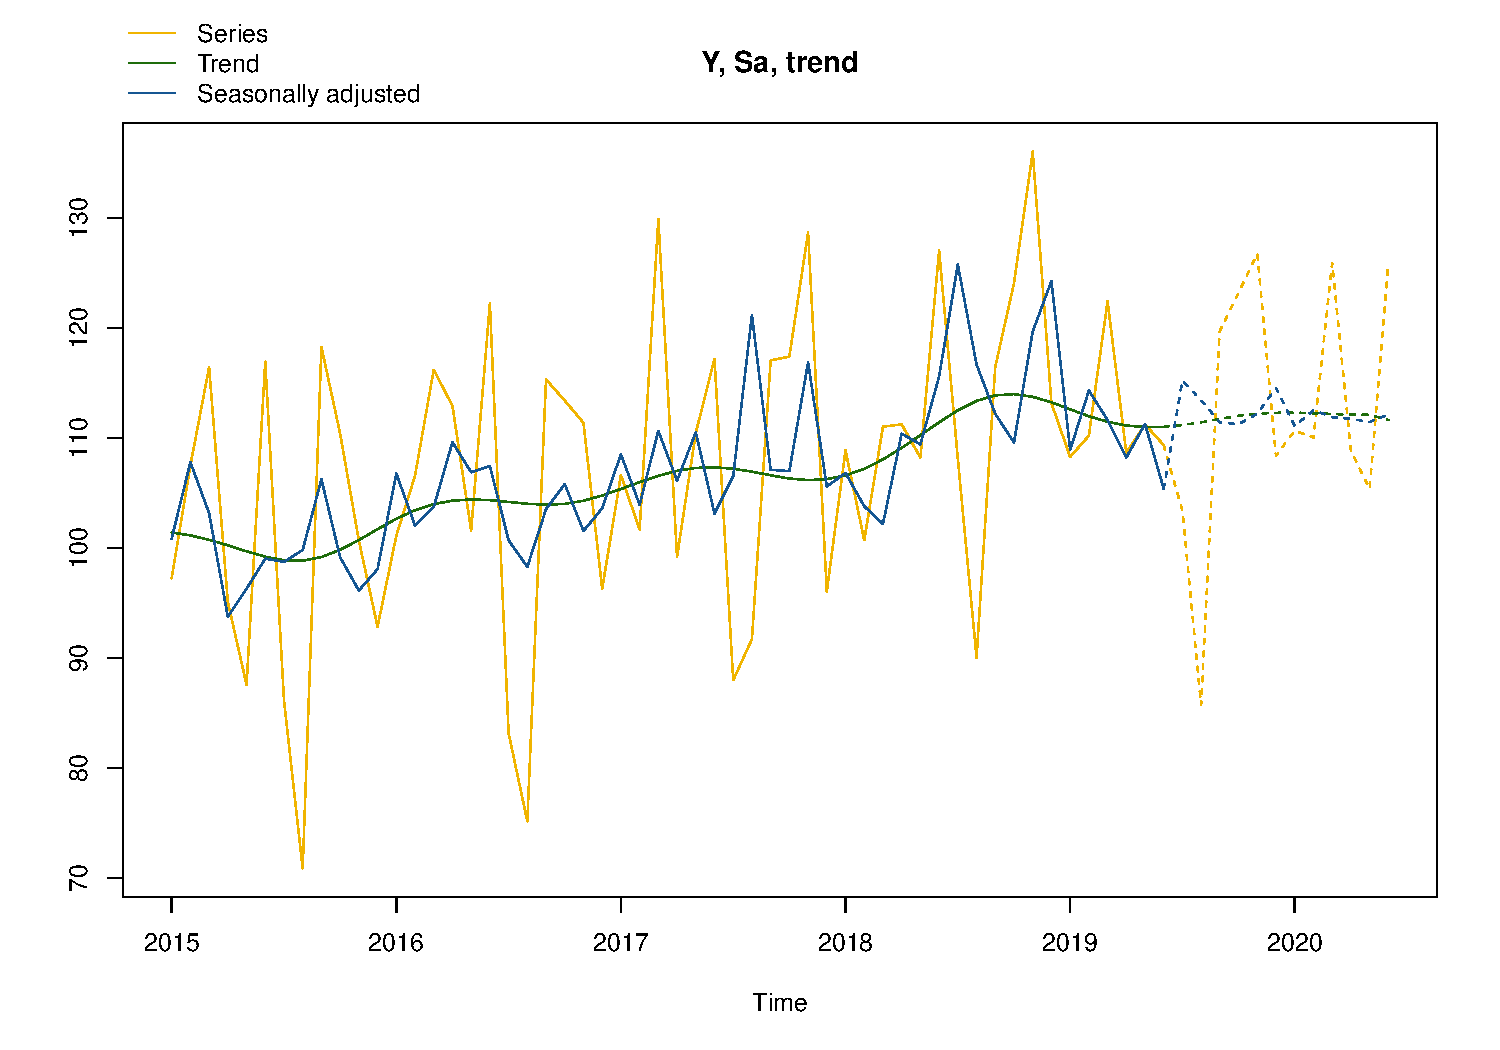
\includegraphics{img/markdown-unnamed-chunk-16-1} \end{center}

\begin{Shaded}
\begin{Highlighting}[]
\CommentTok{\#plot(sa\_x13\_v2, type = "cal{-}seas{-}irr", first\_date = c(2015, 1))}
\end{Highlighting}
\end{Shaded}
\end{frame}

\begin{frame}[fragile,allowframebreaks]{Plots and data visualisation in
version 2}
\protect\hypertarget{plots-and-data-visualisation-in-version-2-2}{}
\begin{Shaded}
\begin{Highlighting}[]
\CommentTok{\# regarima}
\FunctionTok{layout}\NormalTok{(}\FunctionTok{matrix}\NormalTok{(}\DecValTok{1}\SpecialCharTok{:}\DecValTok{6}\NormalTok{, }\DecValTok{3}\NormalTok{, }\DecValTok{2}\NormalTok{))}
\FunctionTok{plot}\NormalTok{(sa\_x13\_v2}\SpecialCharTok{$}\NormalTok{regarima, }\AttributeTok{ask =} \ConstantTok{FALSE}\NormalTok{)}
\end{Highlighting}
\end{Shaded}

\begin{center}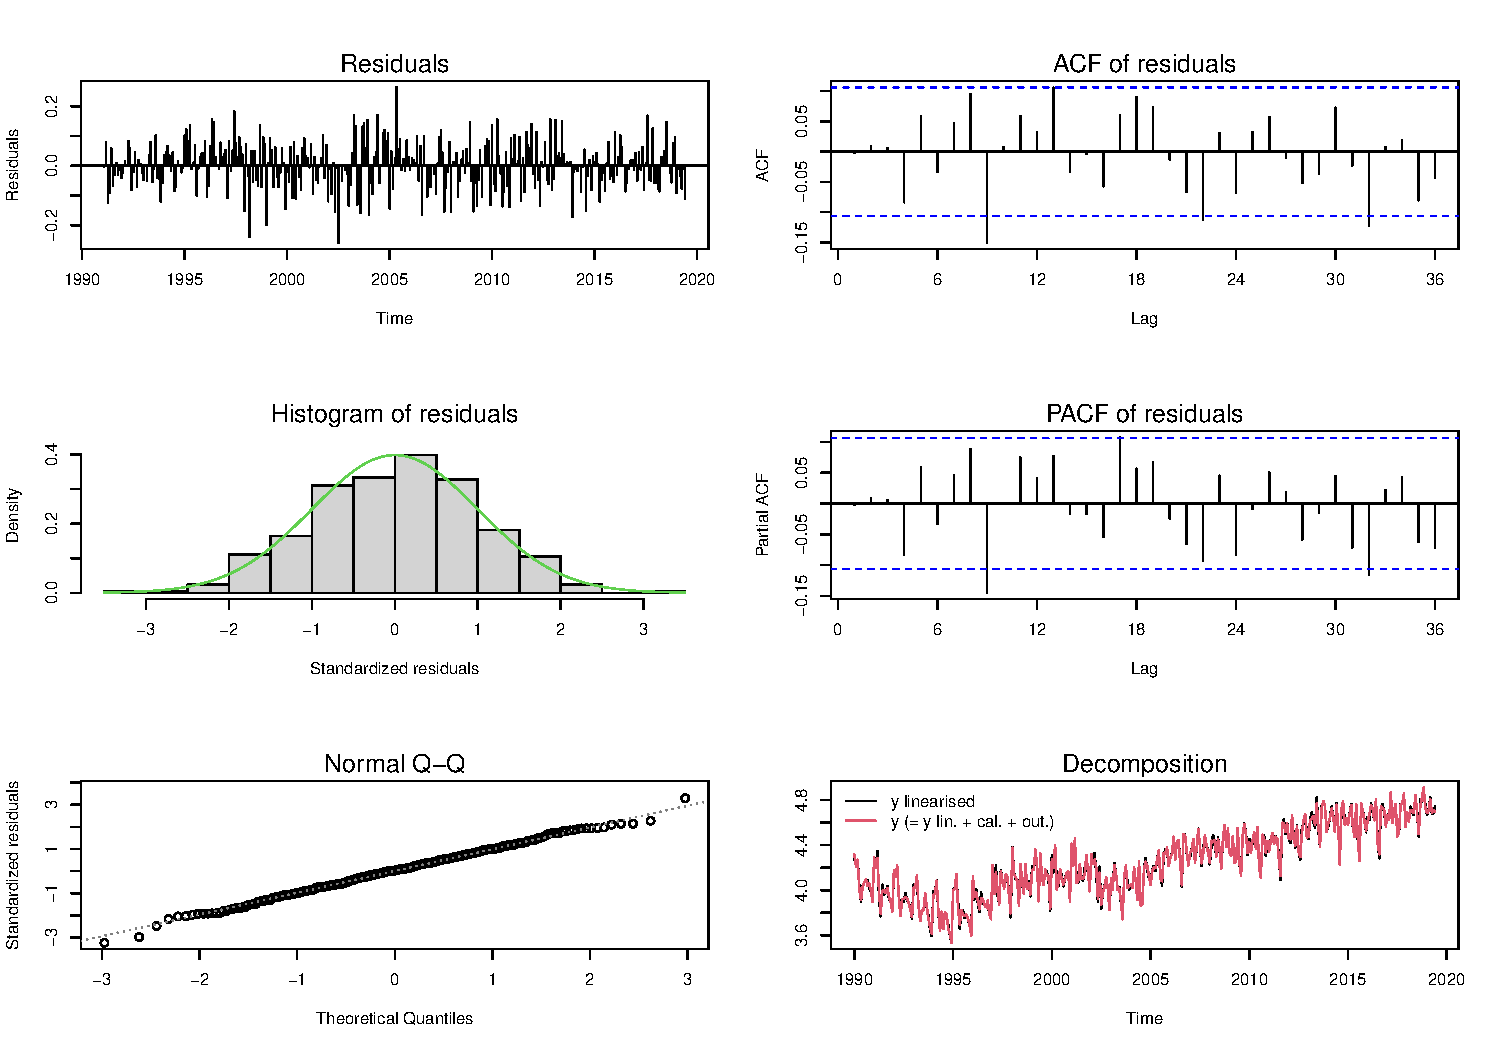
\includegraphics{img/markdown-unnamed-chunk-17-1} \end{center}

\begin{Shaded}
\begin{Highlighting}[]
\CommentTok{\# Plotting SI ratios  }
\FunctionTok{plot}\NormalTok{(sa\_x13\_v2}\SpecialCharTok{$}\NormalTok{decomposition, }\AttributeTok{first\_date =} \FunctionTok{c}\NormalTok{(}\DecValTok{2015}\NormalTok{, }\DecValTok{1}\NormalTok{))}
\end{Highlighting}
\end{Shaded}

\begin{center}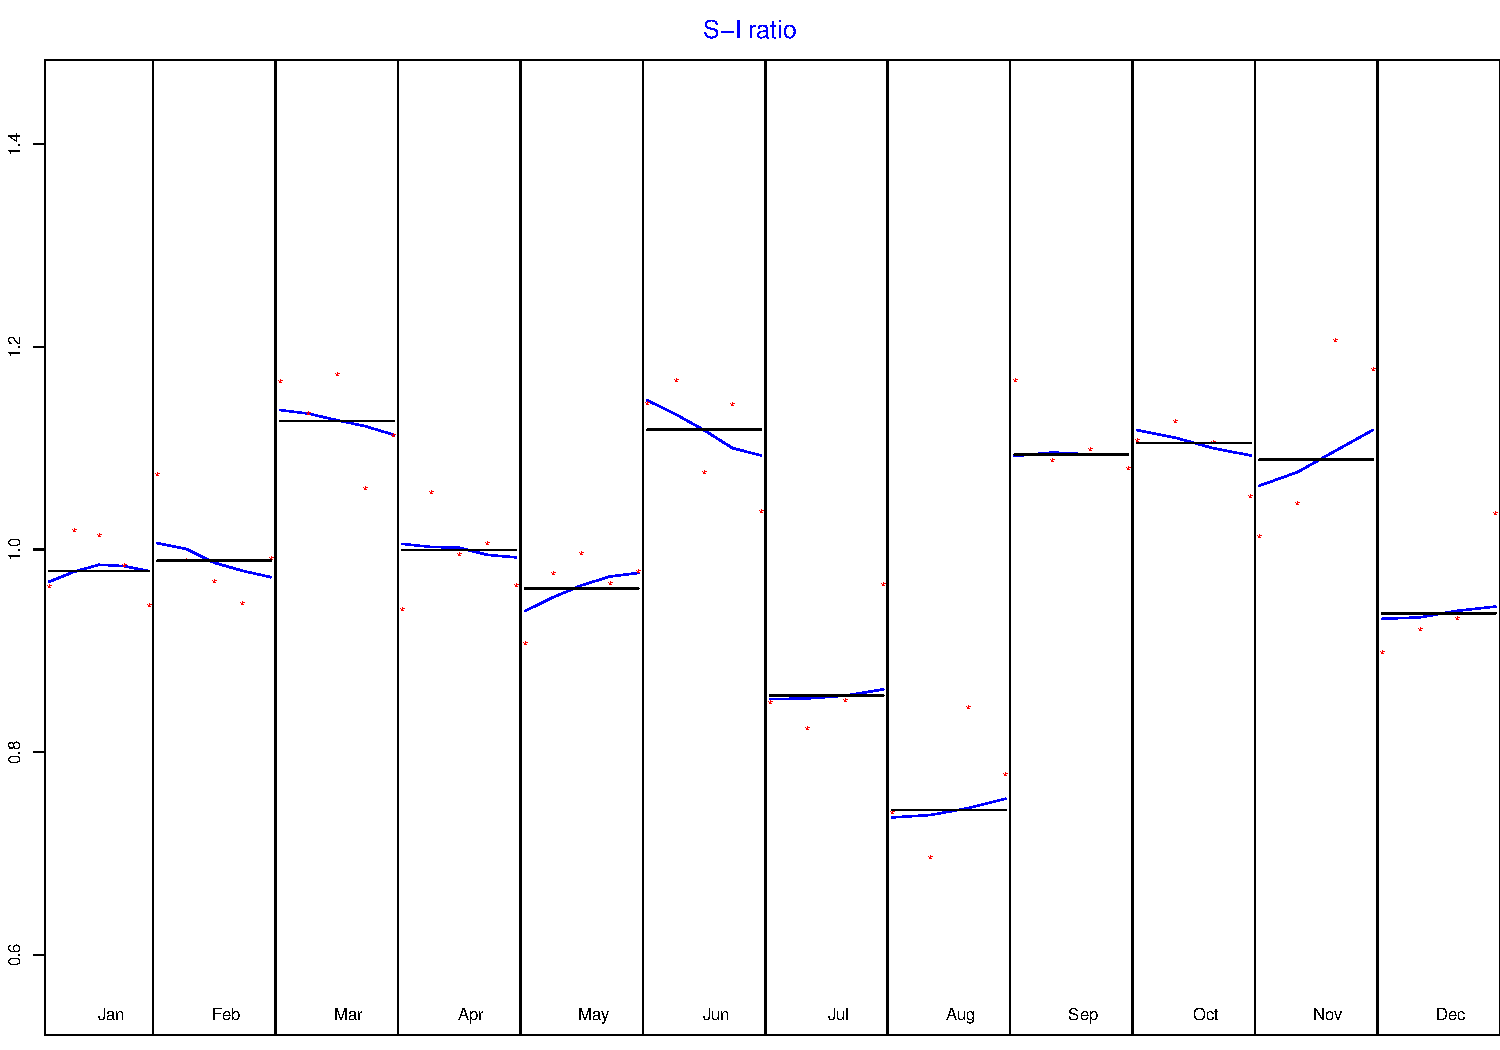
\includegraphics{img/markdown-unnamed-chunk-17-2} \end{center}
\end{frame}

\begin{frame}[fragile,allowframebreaks]{Plots and data visualisation in
version 2}
\protect\hypertarget{plots-and-data-visualisation-in-version-2-3}{}
\begin{Shaded}
\begin{Highlighting}[]
\CommentTok{\# Plotting SI ratios  }
\FunctionTok{plot}\NormalTok{(sa\_x13\_v2}\SpecialCharTok{$}\NormalTok{decomposition, }\AttributeTok{first\_date =} \FunctionTok{c}\NormalTok{(}\DecValTok{2015}\NormalTok{, }\DecValTok{1}\NormalTok{))}
\end{Highlighting}
\end{Shaded}

\begin{center}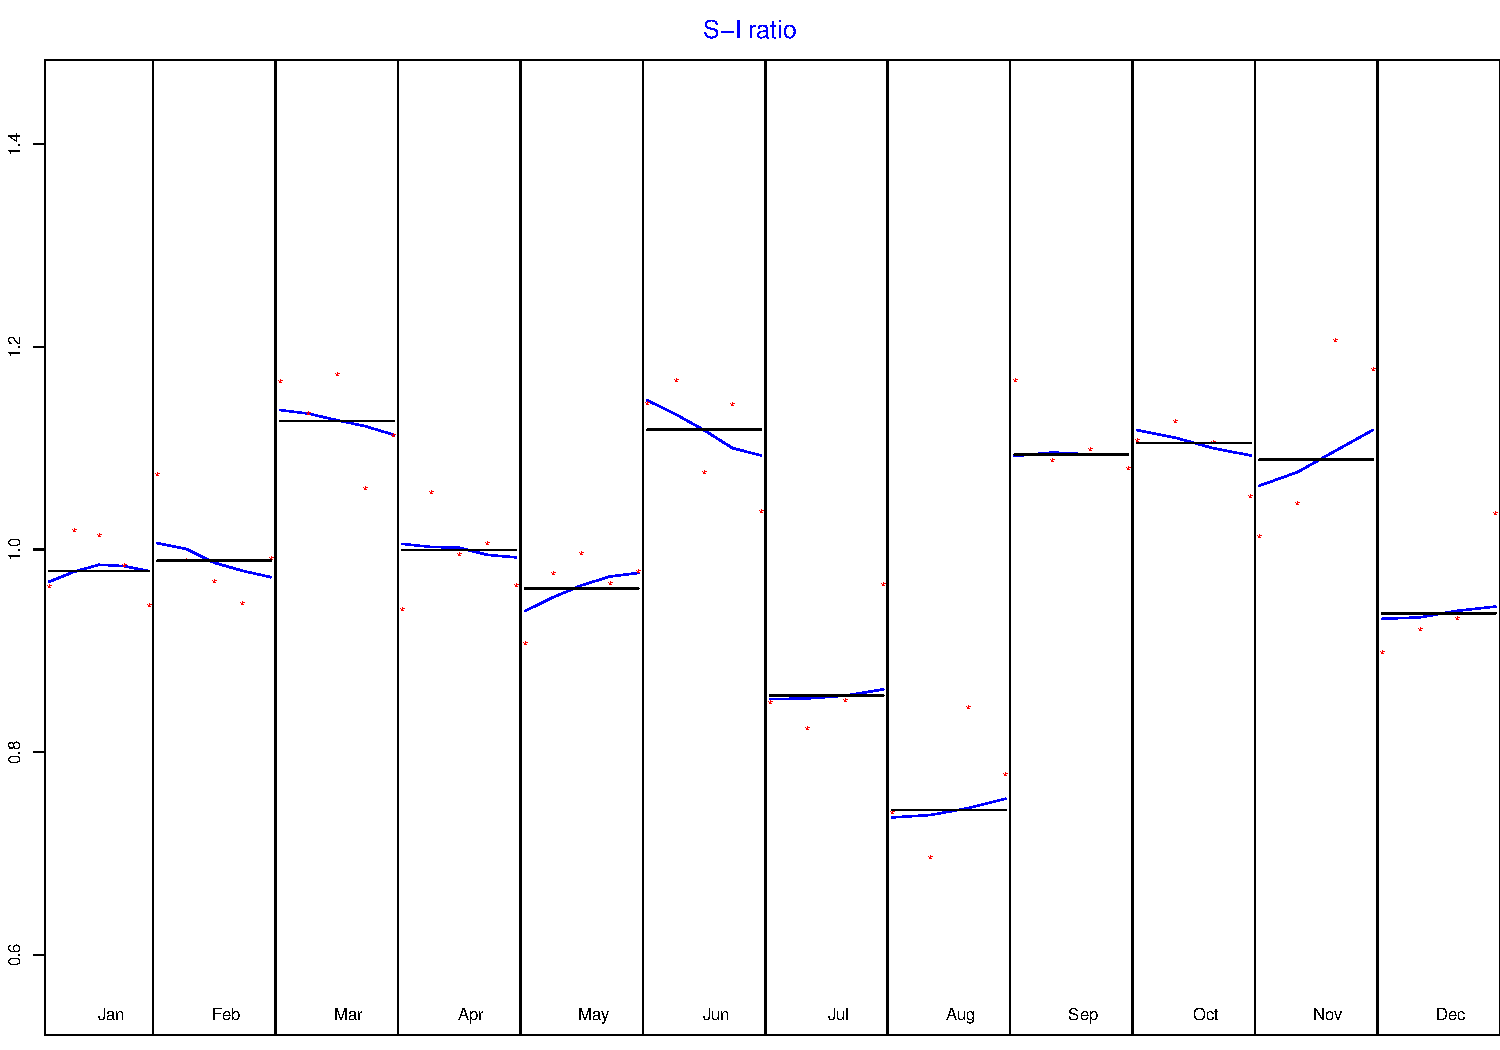
\includegraphics{img/markdown-unnamed-chunk-18-1} \end{center}
\end{frame}

\begin{frame}[fragile,allowframebreaks]{Plots and data visualisation in
version 3}
\protect\hypertarget{plots-and-data-visualisation-in-version-3}{}
In version 3

\begin{itemize}
\item
  final + NEW ``autoplot'' layout
\item
  regarima not available (yet ?)
\item
  SI ratios + NEW ggplot layout
\end{itemize}

\footnotesize

\begin{Shaded}
\begin{Highlighting}[]
\CommentTok{\# version 3}
\CommentTok{\# remotes::install\_github("AQLT/ggdemetra3", INSTALL\_opts = "{-}{-}no{-}multiarch")}
\FunctionTok{library}\NormalTok{(}\StringTok{"ggdemetra3"}\NormalTok{)}
\NormalTok{ggdemetra3}\SpecialCharTok{::}\FunctionTok{siratioplot}\NormalTok{(sa\_x13\_v3)}
\end{Highlighting}
\end{Shaded}

\begin{center}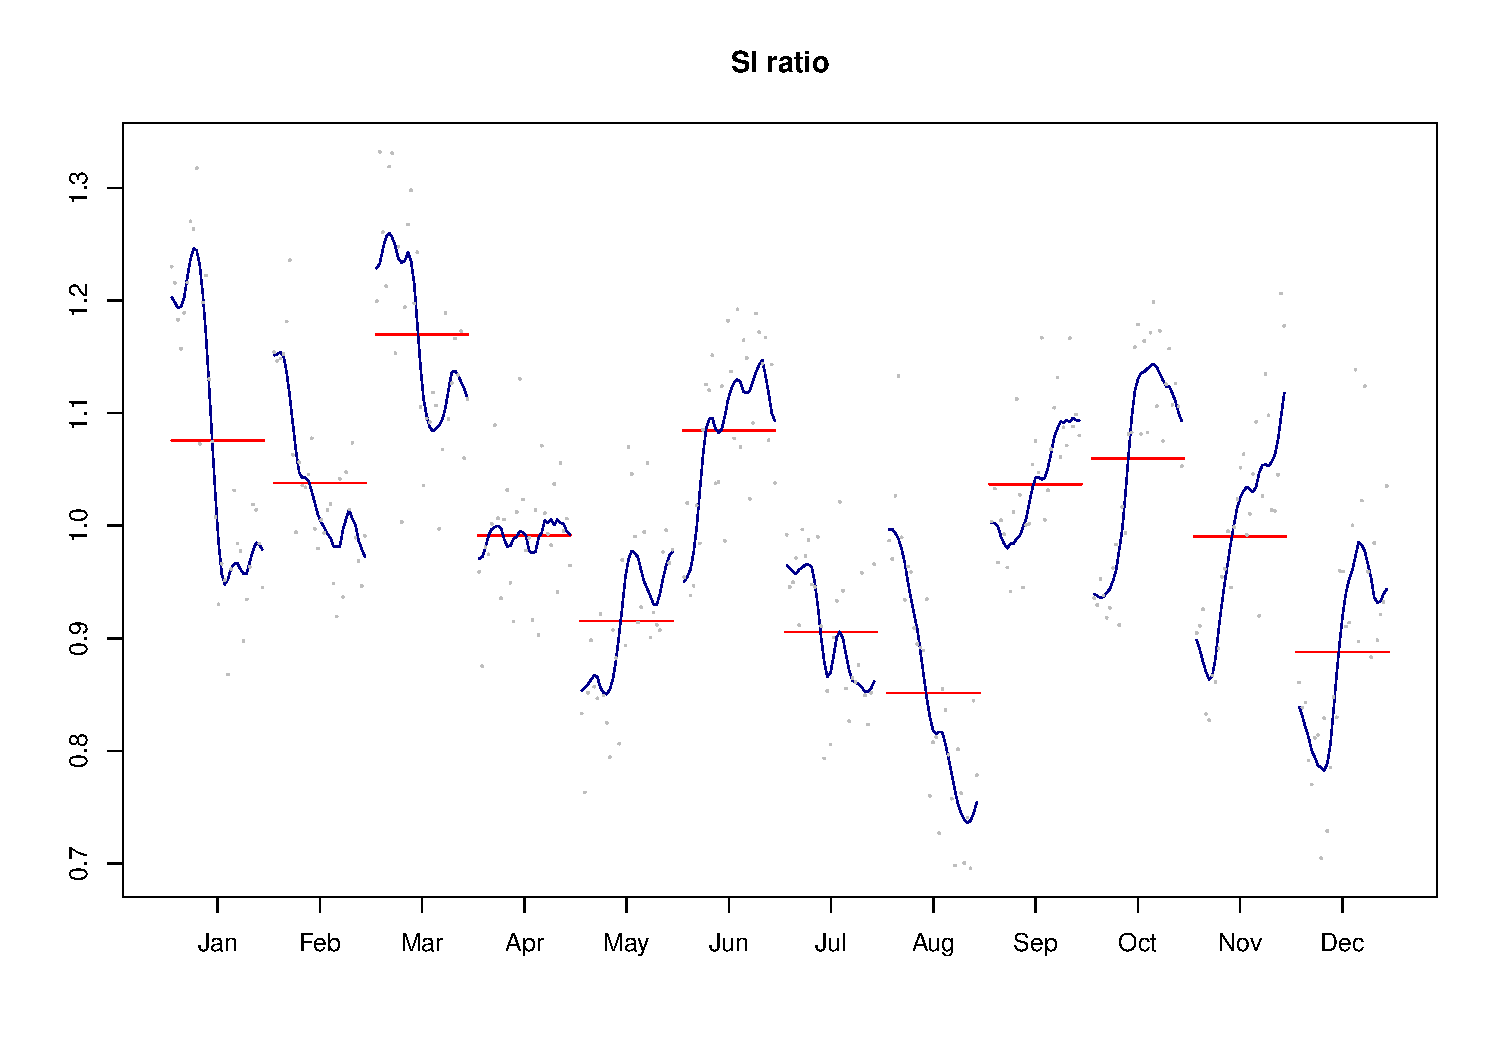
\includegraphics{img/markdown-unnamed-chunk-19-1} \end{center}
\end{frame}

\begin{frame}[fragile,allowframebreaks]{Plots and data visualisation in
version 3}
\protect\hypertarget{plots-and-data-visualisation-in-version-3-1}{}
\begin{Shaded}
\begin{Highlighting}[]
\CommentTok{\# version 3}
\NormalTok{ggdemetra3}\SpecialCharTok{::}\FunctionTok{ggsiratioplot}\NormalTok{(sa\_x13\_v3)}
\end{Highlighting}
\end{Shaded}

\begin{center}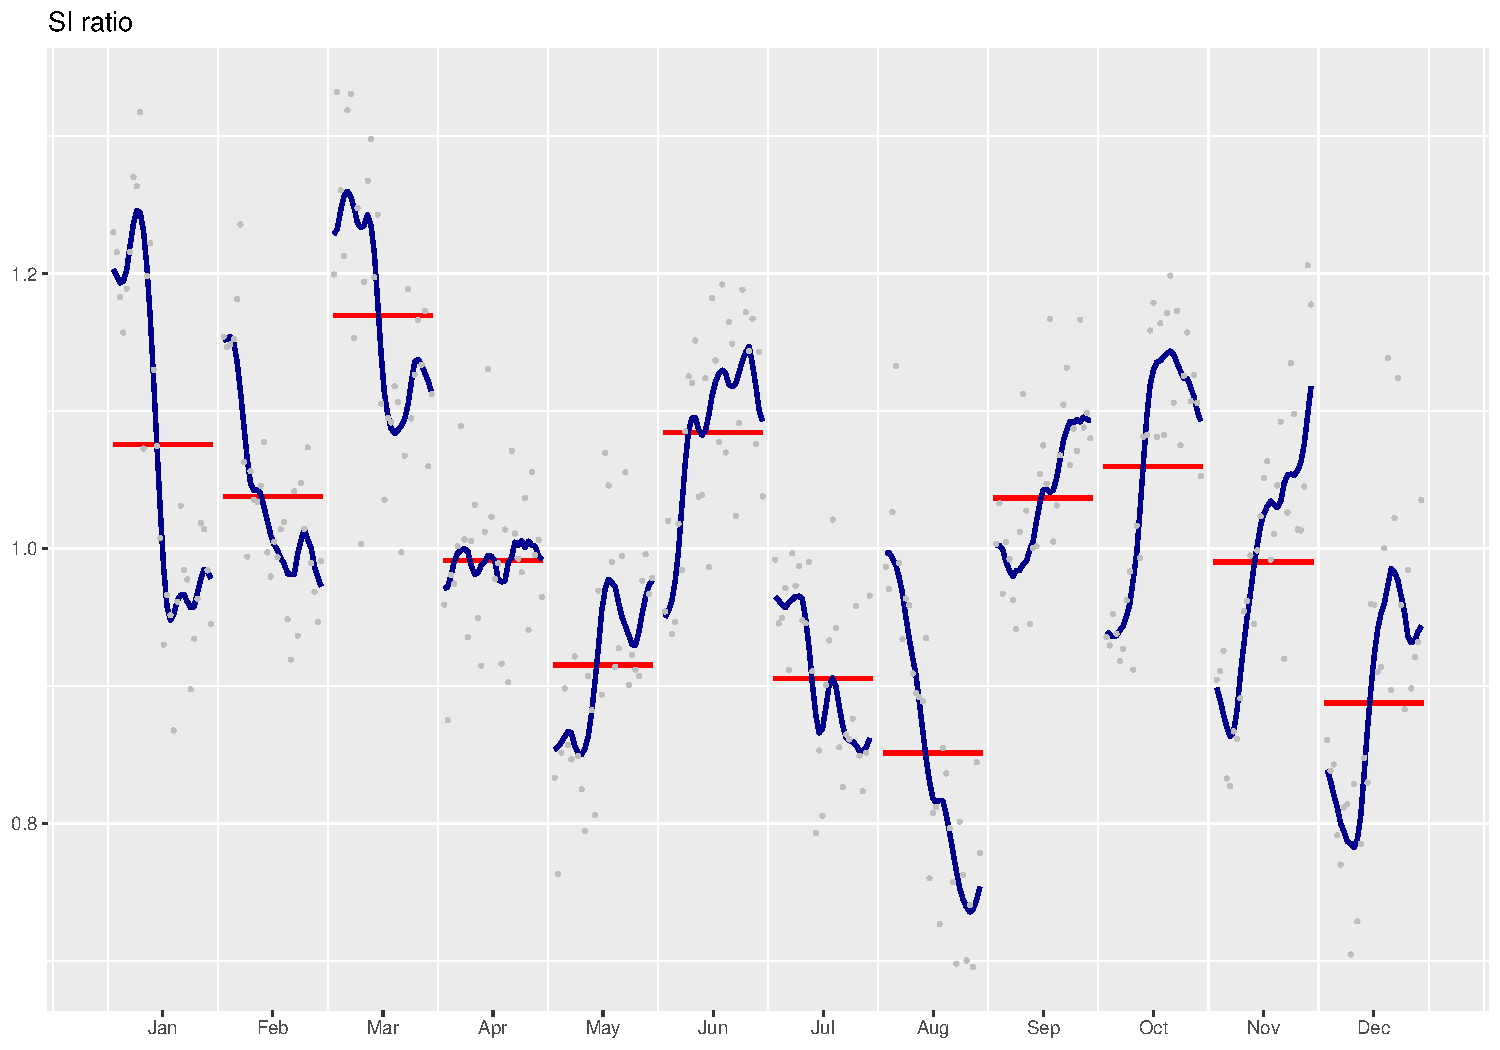
\includegraphics{img/markdown-unnamed-chunk-20-1} \end{center}
\end{frame}

\begin{frame}[fragile,allowframebreaks]{Plots and data visualisation in
version 3}
\protect\hypertarget{plots-and-data-visualisation-in-version-3-2}{}
\begin{Shaded}
\begin{Highlighting}[]
\CommentTok{\# version 3}
\NormalTok{ggplot2}\SpecialCharTok{::}\FunctionTok{autoplot}\NormalTok{(sa\_x13\_v3)}
\end{Highlighting}
\end{Shaded}

\begin{center}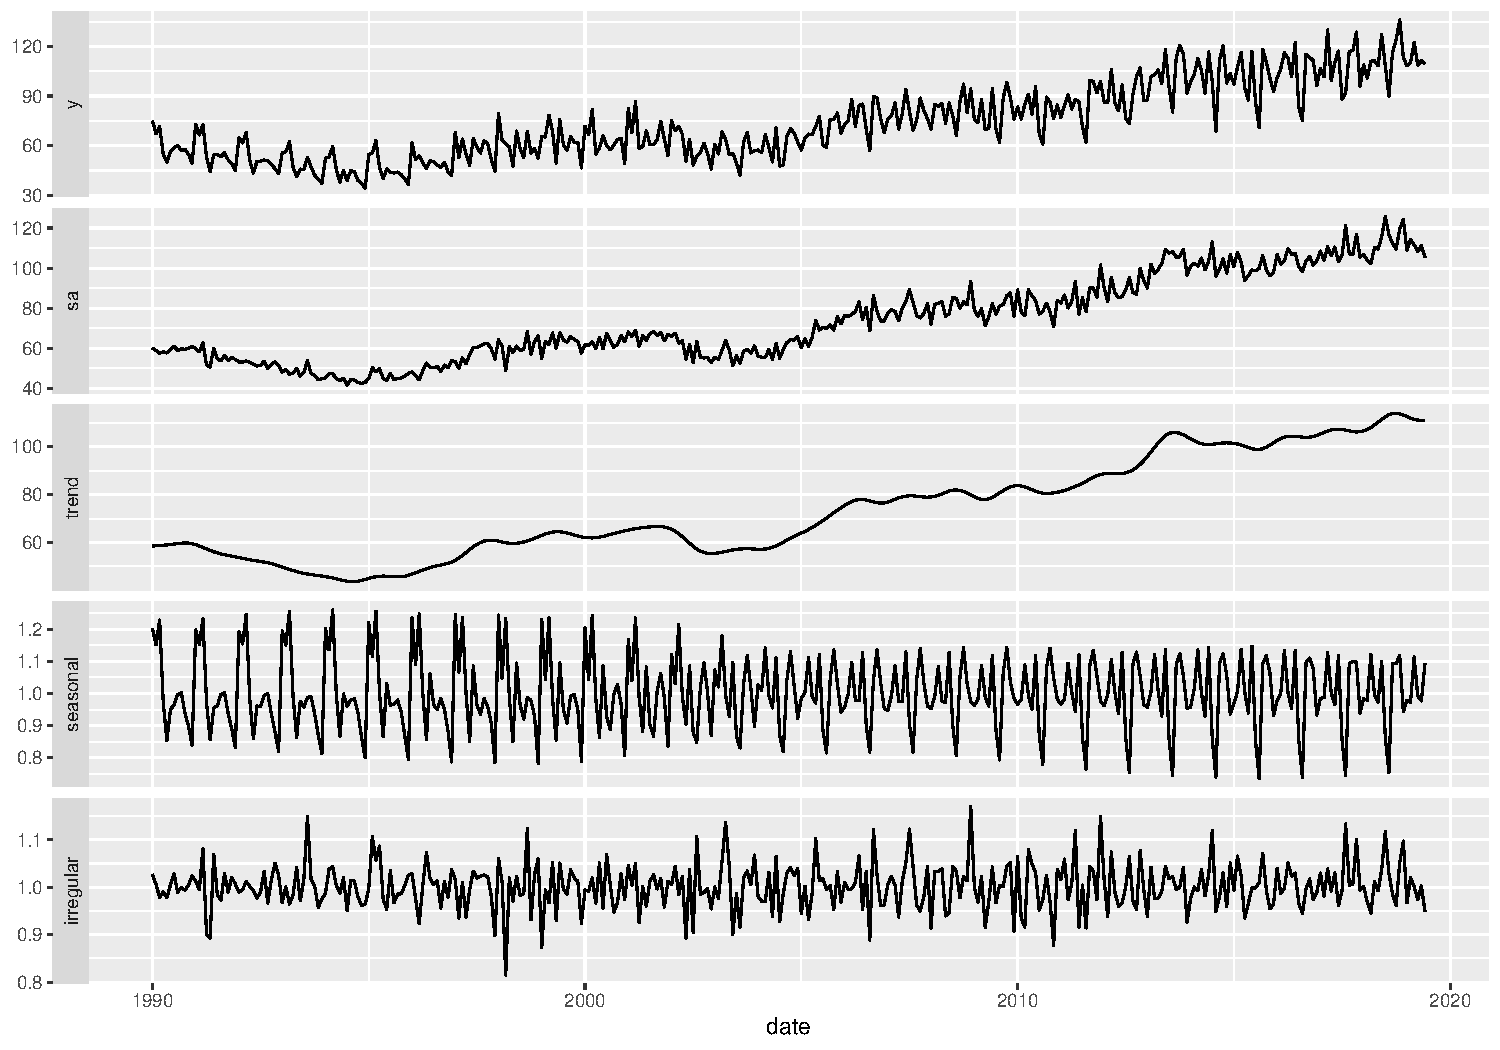
\includegraphics{img/markdown-unnamed-chunk-21-1} \end{center}
\end{frame}

\hypertarget{customizing-specifications}{%
\subsection{Customizing
specifications}\label{customizing-specifications}}

\begin{frame}{Customizing specifications: general steps}
\protect\hypertarget{customizing-specifications-general-steps}{}
To customize a specification you must

\begin{itemize}
\item
  start with a valid specification, usually one of the default specs
  (equivalent to cloning a spec in GUI)
\item
  create a new specification
\item
  apply the new specification to your raw series
\end{itemize}

Some differences between v2 and v3
\end{frame}

\begin{frame}[fragile]{Customizing specifications in version 2}
\protect\hypertarget{customizing-specifications-in-version-2}{}
Direct parameter modification as arguments of the specification function

\footnotesize

\begin{Shaded}
\begin{Highlighting}[]
\CommentTok{\# version 2}
\CommentTok{\# changing estimation span, imposing additive model and}
\CommentTok{\#adding user defined ouliers }
\CommentTok{\# first create a new spec modifying the previous one }
\NormalTok{spec\_1 }\OtherTok{\textless{}{-}} \FunctionTok{x13\_spec}\NormalTok{(sa\_x13\_v2)}
\NormalTok{spec\_2 }\OtherTok{\textless{}{-}} \FunctionTok{x13\_spec}\NormalTok{(spec\_1, }\AttributeTok{estimate.from =} \StringTok{"2004{-}01{-}01"}\NormalTok{,}
                  \AttributeTok{usrdef.outliersEnabled =} \ConstantTok{TRUE}\NormalTok{,}
                             \AttributeTok{usrdef.outliersType =} \FunctionTok{c}\NormalTok{(}\StringTok{"LS"}\NormalTok{, }\StringTok{"AO"}\NormalTok{),}
                             \AttributeTok{usrdef.outliersDate =} \FunctionTok{c}\NormalTok{(}\StringTok{"2008{-}10{-}01"}\NormalTok{, }\StringTok{"2018{-}01{-}01"}\NormalTok{),}
                             \AttributeTok{transform.function =} \StringTok{"None"}\NormalTok{) }\CommentTok{\# additive model}
\CommentTok{\# here the reg{-}arima model will be estimated from  "2004{-}01{-}01" }
\CommentTok{\# the decomposition will be run on the whole span }

\CommentTok{\# new sa processing}
\NormalTok{sa\_x13\_v2\_2 }\OtherTok{\textless{}{-}}\NormalTok{ RJDemetra}\SpecialCharTok{::}\FunctionTok{x13}\NormalTok{(y\_raw, spec\_2)}
\NormalTok{sa\_x13\_v2\_2}\SpecialCharTok{$}\NormalTok{final}\SpecialCharTok{$}\NormalTok{series}
\end{Highlighting}
\end{Shaded}
\end{frame}

\begin{frame}[fragile]{Customizing specifications in version 3}
\protect\hypertarget{customizing-specifications-in-version-3}{}
Use direct and specific \texttt{set\_} functions - for the preprocessing
step (functions defined in \texttt{rjd3modelling}):

\texttt{set\_arima()}, \texttt{set\_automodel()}, \texttt{set\_basic()},
\texttt{set\_easter()}, \texttt{set\_estimate()},
\texttt{set\_outlier()}, \texttt{set\_tradingdays()},
\texttt{set\_transform()}, \texttt{add\_outlier()} and
\texttt{remove\_outlier()}, \texttt{add\_ramp()} and
\texttt{remove\_ramp()}, \texttt{add\_usrdefvar()}

\begin{itemize}
\item
  for the decomposition step in X13 (function defined in
  \texttt{rjd3x13}): \texttt{set\_x11()}
\item
  for the decomposition step in Tramo-Seats (function defined in
  \texttt{rjd3tramoseats}): \texttt{set\_seats()}
\item
  for the benchmarking step (function defined in
  \texttt{rjd3modelling}): \texttt{set\_benchmarking()}
\end{itemize}

Benchmarking New v3 feature, same options available as in GUI.
\end{frame}

\begin{frame}[fragile]{Customizing specifications in version 3: example}
\protect\hypertarget{customizing-specifications-in-version-3-example}{}
\footnotesize

\begin{Shaded}
\begin{Highlighting}[]
\CommentTok{\# start with default spec }
\NormalTok{spec\_1 }\OtherTok{\textless{}{-}} \FunctionTok{spec\_x13\_default}\NormalTok{(}\StringTok{"RSA3"}\NormalTok{)}
\CommentTok{\# or start with existing spec (no extraction function needed)}
\NormalTok{spec\_1 }\OtherTok{\textless{}{-}}\NormalTok{ sa\_x13\_v3\_UD}\SpecialCharTok{$}\NormalTok{estimation\_spec}

\CommentTok{\# set a new spec}
\DocumentationTok{\#\# add outliers }
\NormalTok{spec\_2 }\OtherTok{\textless{}{-}}\NormalTok{ rjd3modelling}\SpecialCharTok{::}\FunctionTok{add\_outlier}\NormalTok{(spec\_1,}
                  \AttributeTok{type =} \FunctionTok{c}\NormalTok{(}\StringTok{"AO"}\NormalTok{), }\FunctionTok{c}\NormalTok{(}\StringTok{"2015{-}01{-}01"}\NormalTok{, }\StringTok{"2010{-}01{-}01"}\NormalTok{))}
\DocumentationTok{\#\# set trading days}
\NormalTok{spec\_2 }\OtherTok{\textless{}{-}}\NormalTok{ rjd3modelling}\SpecialCharTok{::}\FunctionTok{set\_tradingdays}\NormalTok{(spec\_2,}
                  \AttributeTok{option =} \StringTok{"workingdays"}\NormalTok{ )}
\CommentTok{\# set x11 options }
\NormalTok{spec\_2 }\OtherTok{\textless{}{-}} \FunctionTok{set\_x11}\NormalTok{(spec\_2, }\AttributeTok{henderson.filter =} \DecValTok{13}\NormalTok{)}
\CommentTok{\# apply with \textasciigrave{}fast.x13\textasciigrave{} (results only)}
\FunctionTok{fast.x13}\NormalTok{(y, spec\_2)}
\end{Highlighting}
\end{Shaded}
\end{frame}

\begin{frame}{Adding user-defined regressors}
\protect\hypertarget{adding-user-defined-regressors}{}
Differences:

In version 2: regressors added directly to the specification

In version 3: new notion of ``context'': an additional concept designed
to add any user defined (non standard, e.g non outlier'') variable
\end{frame}

\begin{frame}[fragile]{Adding user-defined regressors in v2}
\protect\hypertarget{adding-user-defined-regressors-in-v2}{}
\footnotesize

\begin{Shaded}
\begin{Highlighting}[]
\CommentTok{\# defining user defined trading days }
\NormalTok{spec\_td }\OtherTok{\textless{}{-}} \FunctionTok{x13\_spec}\NormalTok{(spec\_1,}
\AttributeTok{tradingdays.option =} \StringTok{"UserDefined"}\NormalTok{,}
\AttributeTok{tradingdays.test =}\StringTok{"None"}\NormalTok{,}
\AttributeTok{usrdef.varEnabled =} \ConstantTok{TRUE}\NormalTok{,}
\CommentTok{\# the user defined variable will be assigned to the calendar component}
\AttributeTok{usrdef.varType=}\StringTok{"Calendar"}\NormalTok{,}
\AttributeTok{usrdef.var=}\NormalTok{td\_regs ) }\CommentTok{\# regressors have to be a single or multiple TS }
\CommentTok{\# new sa processing}
\NormalTok{sa\_x13\_v2\_4 }\OtherTok{\textless{}{-}} \FunctionTok{x13}\NormalTok{(y\_raw, spec\_td)}
\CommentTok{\# user defined intervention variable  }
\NormalTok{spec\_int }\OtherTok{\textless{}{-}} \FunctionTok{x13\_spec}\NormalTok{(spec\_1,}
                   \AttributeTok{usrdef.varEnabled =} \ConstantTok{TRUE}\NormalTok{,}
                   \CommentTok{\# the user defined variable will be assigned to the trend component}
                   \AttributeTok{usrdef.varType =} \StringTok{"Trend"}\NormalTok{,}
                   \AttributeTok{usrdef.var =}\NormalTok{ x ) }\CommentTok{\# x has to to be a single or multiple TS }
\CommentTok{\# new sa processing}
\NormalTok{sa\_x13\_v2\_5 }\OtherTok{\textless{}{-}} \FunctionTok{x13}\NormalTok{(y\_raw, spec\_int)}
\end{Highlighting}
\end{Shaded}
\end{frame}

\begin{frame}[fragile]{Adding user-defined regressors in version 3}
\protect\hypertarget{adding-user-defined-regressors-in-version-3}{}
\footnotesize

\begin{Shaded}
\begin{Highlighting}[]
\CommentTok{\# define a user defined trading days regressor }
\NormalTok{td\_reg1 }\OtherTok{\textless{}{-}}\NormalTok{ rjd3modelling}\SpecialCharTok{::}\FunctionTok{td}\NormalTok{(}\DecValTok{12}\NormalTok{, }\AttributeTok{start =} \FunctionTok{start}\NormalTok{(y\_raw), }\AttributeTok{length =} \FunctionTok{length}\NormalTok{(y\_raw), }\AttributeTok{groups =} \FunctionTok{c}\NormalTok{(}\DecValTok{1}\NormalTok{, }\DecValTok{1}\NormalTok{, }\DecValTok{1}\NormalTok{, }\DecValTok{1}\NormalTok{, }\DecValTok{1}\NormalTok{, }\DecValTok{0}\NormalTok{, }\DecValTok{0}\NormalTok{))}

\CommentTok{\# define a context}
\NormalTok{my\_context }\OtherTok{\textless{}{-}}\NormalTok{ rjd3modelling}\SpecialCharTok{::}\FunctionTok{modelling\_context}\NormalTok{(}\AttributeTok{variables =} \FunctionTok{list}\NormalTok{(}\AttributeTok{a =}\NormalTok{ xvar))}

\CommentTok{\# set a new specification from a default specification}
\NormalTok{spec\_td }\OtherTok{\textless{}{-}}\NormalTok{ rjd3x13}\SpecialCharTok{::}\FunctionTok{spec\_regarima\_default}\NormalTok{(}\AttributeTok{name =} \StringTok{"rg3"}\NormalTok{) }\SpecialCharTok{|\textgreater{}}
\NormalTok{  rjd3modelling}\SpecialCharTok{::}\FunctionTok{add\_usrdefvar}\NormalTok{(}\AttributeTok{id =} \StringTok{"r.a"}\NormalTok{)}

\CommentTok{\# new reg{-}arima estimation}
\NormalTok{reg\_a\_estimation }\OtherTok{\textless{}{-}}\NormalTok{ rjd3x13}\SpecialCharTok{::}\FunctionTok{regarima}\NormalTok{(}\FunctionTok{window}\NormalTok{(ts, }\AttributeTok{start =} \DecValTok{1985}\NormalTok{, }\AttributeTok{end =} \DecValTok{2013}\NormalTok{), spec\_td, }\AttributeTok{context =}\NormalTok{ my\_context)}
\end{Highlighting}
\end{Shaded}
\end{frame}

\hypertarget{refreshing-data}{%
\subsection{Refreshing data}\label{refreshing-data}}

\begin{frame}[fragile]{Refreshing data: Estimation\_spec vs result\_spec
(1/2)}
\protect\hypertarget{refreshing-data-estimation_spec-vs-result_spec-12}{}
Possibility of refreshing data is a NEW feature of version 3.

In the ``sa\_model'' object generated by the estimation process:

\begin{itemize}
\item
  specification is separated from results
\item
  split in ``estimation\_spec'' (domain spec): set of customizable
  constraints
\item
  and ``result\_spec'' (point spec)
\end{itemize}

\footnotesize

\begin{Shaded}
\begin{Highlighting}[]
\NormalTok{sa\_x13\_v3}\SpecialCharTok{$}\NormalTok{estimation\_spec}\SpecialCharTok{$}\NormalTok{regarima}\SpecialCharTok{$}\NormalTok{arima}
\end{Highlighting}
\end{Shaded}

\begin{verbatim}
- result spec (or point spec)
\end{verbatim}

\footnotesize

\begin{Shaded}
\begin{Highlighting}[]
\NormalTok{sa\_x13\_v3}\SpecialCharTok{$}\NormalTok{result\_spec}\SpecialCharTok{$}\NormalTok{regarima}\SpecialCharTok{$}\NormalTok{arima}
\end{Highlighting}
\end{Shaded}
\end{frame}

\begin{frame}[fragile]{Estimation\_spec vs result\_spec}
\protect\hypertarget{estimation_spec-vs-result_spec}{}
\begin{itemize}
\item
  in v2 could only retrieve a (point) result\_spec (extracted with
  \texttt{x13\_spec()} for example)
\item
  in v3 your are able to re-estimate the ``result\_spec'' inside a
  domain of constraints (estimation spec), freeing restrictions on
  selected parameters: just like in GUI, or Cruncher.
\end{itemize}
\end{frame}

\begin{frame}[fragile]{Steps for refreshing data}
\protect\hypertarget{steps-for-refreshing-data}{}
\footnotesize

\begin{Shaded}
\begin{Highlighting}[]
\NormalTok{current\_result\_spec }\OtherTok{\textless{}{-}}\NormalTok{ sa\_x13\_v3}\SpecialCharTok{$}\NormalTok{result\_spec}
\NormalTok{current\_domain\_spec }\OtherTok{\textless{}{-}}\NormalTok{ sa\_x13\_v3}\SpecialCharTok{$}\NormalTok{estimation\_spec}

\CommentTok{\# generate NEW spec for refresh }
\NormalTok{refreshed\_spec }\OtherTok{\textless{}{-}} \FunctionTok{x13.refresh}\NormalTok{(current\_result\_spec, }\CommentTok{\# point spec to be refreshed}
\NormalTok{            current\_domain\_spec, }\CommentTok{\#domain spec (set of constraints)}
            \AttributeTok{policy =} \StringTok{"Outliers"}\NormalTok{,}
            \AttributeTok{period =} \DecValTok{12}\NormalTok{, }\CommentTok{\# monthly series}
            \AttributeTok{start =} \StringTok{"2017{-}01{-}01"}\NormalTok{,}
            \AttributeTok{end =} \ConstantTok{NULL}\NormalTok{)}

\CommentTok{\# apply the new spec on new data : y\_new= y\_raw + 1 month}

\NormalTok{sa\_x13\_v3\_refresh }\OtherTok{\textless{}{-}} \FunctionTok{x13}\NormalTok{(y\_new, refreshed\_spec)}
\end{Highlighting}
\end{Shaded}

Outliers identification : more flexible than ``last outliers'' or ``all
outliers'' in v2, here the span can be customized .

(Warning: x13.refresh hasn't been thoroughly tested yet)
\end{frame}

\begin{frame}{Refresh Policies}
\protect\hypertarget{refresh-policies}{}
\begin{itemize}
\tightlist
\item
  ``FreeParameters'' : all reset to default
\item
  ``Complete'': all reset to default but user defined stored
\item
  ``Outliers\_StochasticComponent''
\item
  ``Outliers''
\item
  ``FixedParameters''
\item
  ``FixedAutoRegressiveParameters'' (for Seats)
\item
  ``Fixed''
\end{itemize}
\end{frame}

\hypertarget{sa-of-high-frequency-data}{%
\section{SA of High-Frequency data}\label{sa-of-high-frequency-data}}

\begin{frame}{SA of High-Frequency data (1/2)}
\protect\hypertarget{sa-of-high-frequency-data-12}{}
Specificity: high-frequency data can display multiple and non integer
periodicities:

For example a daily series might display 3 periodicities: - weekly
(\(p=7\)): Mondays are alike and different from Sundays (DOW) -
intra-monthly (\(p=30.44\)): the last days of each month are different
from the first ones (DOM) - yearly (\(p=365.25\)): from on year to
another the 15th of June are alike, summer days are alike (DOY)

Two classes of solutions: - round periodicities (might involve imputing
data) (extended STL,..) - use approximations for fractional backshift
powers (extended X13-Arima and Tramo-Seats)
\end{frame}

\begin{frame}{SA of High-Frequency data (2/2)}
\protect\hypertarget{sa-of-high-frequency-data-22}{}
\begin{itemize}
\tightlist
\item
  Specific tools:\\
  rjd3highfreq and rjd3stl (version 3) (version 2 : rjdhighfreq)
\end{itemize}

Different data format: numeric vectors (and NOT TS objects)

\begin{itemize}
\item
  linerarization with \textbf{fractional airline model} (correction for
  calendar effects and outlier detection)
\item
  iterative decomposition (extended X-11 and Seats) starting with the
  highest frequency
\end{itemize}

(See presentation about rjd3highfreq in Webinar GitHub Repo)
\end{frame}

\begin{frame}[fragile]{Linearization: code template}
\protect\hypertarget{linearization-code-template}{}
\footnotesize

\begin{Shaded}
\begin{Highlighting}[]
\NormalTok{rjd3highfreq}\SpecialCharTok{::}\NormalTok{fractionalAirlineEstimation}
\NormalTok{                        (df\_daily}\SpecialCharTok{$}\NormalTok{log\_births, }\CommentTok{\# here series in log}
                \AttributeTok{x =}\NormalTok{ q, }\CommentTok{\# q= calendar}
                \AttributeTok{periods =} \DecValTok{7}\NormalTok{, }\CommentTok{\# approx  c(7,365.25)}
                \AttributeTok{ndiff =} \DecValTok{2}\NormalTok{, }\AttributeTok{ar =} \ConstantTok{FALSE}\NormalTok{, }\AttributeTok{mean =} \ConstantTok{FALSE}\NormalTok{,}
                \AttributeTok{outliers =} \FunctionTok{c}\NormalTok{(}\StringTok{"ao"}\NormalTok{,}\StringTok{"wo"}\NormalTok{,}\StringTok{"LS"}\NormalTok{), }
                \CommentTok{\# WO compensation}
                \AttributeTok{criticalValue =} \DecValTok{0}\NormalTok{, }\CommentTok{\# computed in the algorithm}
                \AttributeTok{precision =} \FloatTok{1e{-}9}\NormalTok{, }\AttributeTok{approximateHessian =} \ConstantTok{TRUE}\NormalTok{)}
                    
\CommentTok{\# calendar regressors can be defined with the rjd3modelling package }
\end{Highlighting}
\end{Shaded}

See \{rjd3highfreq\} help pages
\end{frame}

\begin{frame}[fragile]{Decomposition with extended X-11: code template}
\protect\hypertarget{decomposition-with-extended-x-11-code-template}{}
\footnotesize

\begin{Shaded}
\begin{Highlighting}[]
\CommentTok{\#step 1: p=7}
\NormalTok{x11.dow }\OtherTok{\textless{}{-}}\NormalTok{ rjd3highfreq}\SpecialCharTok{::}\FunctionTok{x11}\NormalTok{(}\FunctionTok{exp}\NormalTok{(pre.mult}\SpecialCharTok{$}\NormalTok{model}\SpecialCharTok{$}\NormalTok{linearized),}
        \AttributeTok{period =} \DecValTok{7}\NormalTok{,                 }\CommentTok{\# DOW pattern}
        \AttributeTok{mul =} \ConstantTok{TRUE}\NormalTok{,                              }
        \AttributeTok{trend.horizon =} \DecValTok{9}\NormalTok{,  }\CommentTok{\# 1/2 Filter length : not too long vs p}
        \AttributeTok{trend.degree =} \DecValTok{3}\NormalTok{,                         }\CommentTok{\# Polynomial degree}
        \AttributeTok{trend.kernel =} \StringTok{"Henderson"}\NormalTok{,               }\CommentTok{\# Kernel function}
        \AttributeTok{trend.asymmetric =} \StringTok{"CutAndNormalize"}\NormalTok{,     }\CommentTok{\# Truncation method}
        \AttributeTok{seas.s0 =} \StringTok{"S3X9"}\NormalTok{, }\AttributeTok{seas.s1 =} \StringTok{"S3X9"}\NormalTok{,       }\CommentTok{\# Seasonal filters}
        \AttributeTok{extreme.lsig =} \FloatTok{1.5}\NormalTok{, }\AttributeTok{extreme.usig =} \FloatTok{2.5}\NormalTok{)   }\CommentTok{\# Sigma{-}limits}
\CommentTok{\#step 2: p=365.25}
\NormalTok{x11.doy }\OtherTok{\textless{}{-}}\NormalTok{ rjd3highfreq}\SpecialCharTok{::}\FunctionTok{x11}\NormalTok{(x11.dow}\SpecialCharTok{$}\NormalTok{decomposition}\SpecialCharTok{$}\NormalTok{sa,  }\CommentTok{\# previous sa}
                    \AttributeTok{period =} \FloatTok{365.2425}\NormalTok{,         }\CommentTok{\# DOY pattern}
                    \AttributeTok{mul =} \ConstantTok{TRUE}\NormalTok{) }\CommentTok{\#other parameters skipped here}
\end{Highlighting}
\end{Shaded}
\end{frame}

\begin{frame}[fragile]{Decomposition with extended Seats: code template}
\protect\hypertarget{decomposition-with-extended-seats-code-template}{}
\footnotesize

\begin{Shaded}
\begin{Highlighting}[]
\CommentTok{\#step 1: p=7}
\CommentTok{\#step 2: p=365.25}
\NormalTok{amb.doy }\OtherTok{\textless{}{-}}\NormalTok{ rjd3highfreq}\SpecialCharTok{::}\FunctionTok{fractionalAirlineDecomposition}\NormalTok{(}
\NormalTok{  amb.dow}\SpecialCharTok{$}\NormalTok{decomposition}\SpecialCharTok{$}\NormalTok{sa,  }\CommentTok{\# DOW{-}adjusted linearised data}
  \AttributeTok{period =} \FloatTok{365.2425}\NormalTok{,         }\CommentTok{\# DOY pattern}
  \AttributeTok{sn =} \ConstantTok{FALSE}\NormalTok{,                }\CommentTok{\# Signal (SA){-}noise decomposition }
  \AttributeTok{stde =} \ConstantTok{FALSE}\NormalTok{,              }\CommentTok{\# Compute standard deviations}
  \AttributeTok{nbcasts =} \DecValTok{0}\NormalTok{, }\AttributeTok{nfcasts =} \DecValTok{0}\NormalTok{)  }\CommentTok{\# Numbers of back{-} and forecasts}
\end{Highlighting}
\end{Shaded}
\end{frame}

\hypertarget{generating-user-defined-auxilary-variables}{%
\section{Generating User-defined auxilary
variables}\label{generating-user-defined-auxilary-variables}}

\hypertarget{calendars}{%
\subsection{Calendars}\label{calendars}}

\begin{frame}{Calendars}
\protect\hypertarget{calendars-1}{}
New features of version 3:

\begin{itemize}
\item
  generating calendars in R (see GUI function in v2)
\item
  generating calendar regressors

  \begin{itemize}
  \tightlist
  \item
    raw number of days or contrasts
  \item
    long term mean correction or not
  \item
    user-defined groups of days
  \item
    user-defined contrast days (associated with holidays)
  \end{itemize}
\end{itemize}

Can be done with rjd3modelling package
\end{frame}

\begin{frame}[fragile]{Creation of a specific calendar}
\protect\hypertarget{creation-of-a-specific-calendar}{}
\footnotesize

\begin{Shaded}
\begin{Highlighting}[]
\FunctionTok{library}\NormalTok{(}\StringTok{"rjd3modelling"}\NormalTok{)}
\CommentTok{\# French}
\NormalTok{fr\_cal }\OtherTok{\textless{}{-}} \FunctionTok{calendar.new}\NormalTok{()}
\FunctionTok{calendar.holiday}\NormalTok{(fr\_cal, }\StringTok{"NEWYEAR"}\NormalTok{)}
\FunctionTok{calendar.holiday}\NormalTok{(fr\_cal, }\StringTok{"EASTERMONDAY"}\NormalTok{)}
\FunctionTok{calendar.holiday}\NormalTok{(fr\_cal, }\StringTok{"MAYDAY"}\NormalTok{)}
\FunctionTok{calendar.fixedday}\NormalTok{(fr\_cal, }\AttributeTok{month =} \DecValTok{5}\NormalTok{, }\AttributeTok{day =} \DecValTok{8}\NormalTok{,}
                  \AttributeTok{start =} \StringTok{"1982{-}01{-}01"}\NormalTok{)}
\CommentTok{\# calendar.holiday(fr\_cal, "WHITMONDAY") \# Equivalent to:}
\FunctionTok{calendar.easter}\NormalTok{(fr\_cal, }\AttributeTok{offset =} \DecValTok{61}\NormalTok{)}

\FunctionTok{calendar.fixedday}\NormalTok{(fr\_cal, }\AttributeTok{month =} \DecValTok{7}\NormalTok{, }\AttributeTok{day =} \DecValTok{14}\NormalTok{)}
\CommentTok{\# calendar.holiday(fr\_cal, "ASSUMPTION")}
\FunctionTok{calendar.easter}\NormalTok{(fr\_cal, }\AttributeTok{offset =} \DecValTok{61}\NormalTok{)}
\FunctionTok{calendar.holiday}\NormalTok{(fr\_cal, }\StringTok{"ALLSAINTSDAY"}\NormalTok{)}
\FunctionTok{calendar.holiday}\NormalTok{(fr\_cal, }\StringTok{"ARMISTICE"}\NormalTok{)}
\FunctionTok{calendar.holiday}\NormalTok{(fr\_cal, }\StringTok{"CHRISTMAS"}\NormalTok{)}
\end{Highlighting}
\end{Shaded}
\end{frame}

\begin{frame}[fragile,allowframebreaks]{Creation of a associated
regressors}
\protect\hypertarget{creation-of-a-associated-regressors}{}
Use \texttt{holidays()} to get the days of the holidays and
\texttt{htd()} to get the trading days regressors

\footnotesize

\begin{Shaded}
\begin{Highlighting}[]
\FunctionTok{holidays}\NormalTok{(fr\_cal, }\StringTok{"2020{-}12{-}24"}\NormalTok{, }\DecValTok{10}\NormalTok{,}\AttributeTok{single =}\NormalTok{ T)}
\end{Highlighting}
\end{Shaded}

\begin{verbatim}
##            [,1]
## 2020-12-24    0
## 2020-12-25    1
## 2020-12-26    0
## 2020-12-27    0
## 2020-12-28    0
## 2020-12-29    0
## 2020-12-30    0
## 2020-12-31    0
## 2021-01-01    1
## 2021-01-02    0
\end{verbatim}

\begin{Shaded}
\begin{Highlighting}[]
\NormalTok{s }\OtherTok{\textless{}{-}} \FunctionTok{ts}\NormalTok{(}\DecValTok{0}\NormalTok{, }\AttributeTok{start =} \DecValTok{2020}\NormalTok{, }\AttributeTok{end =} \FunctionTok{c}\NormalTok{(}\DecValTok{2020}\NormalTok{, }\DecValTok{11}\NormalTok{), }\AttributeTok{frequency =} \DecValTok{12}\NormalTok{)}
\CommentTok{\# Trading{-}days regressors (each day has a different effect, sunday as contrasts)}
\NormalTok{td\_reg }\OtherTok{\textless{}{-}} \FunctionTok{htd}\NormalTok{(fr\_cal, }\AttributeTok{s =}\NormalTok{ s, }\AttributeTok{groups =} \FunctionTok{c}\NormalTok{(}\DecValTok{1}\NormalTok{, }\DecValTok{2}\NormalTok{, }\DecValTok{3}\NormalTok{, }\DecValTok{4}\NormalTok{, }\DecValTok{5}\NormalTok{, }\DecValTok{6}\NormalTok{, }\DecValTok{0}\NormalTok{))}
\CommentTok{\# Working{-}days regressors (Monday = ... = Friday; Saturday = Sunday = contrasts)}
\NormalTok{wd\_reg }\OtherTok{\textless{}{-}} \FunctionTok{htd}\NormalTok{(fr\_cal, }\AttributeTok{s =}\NormalTok{ s, }\AttributeTok{groups =} \FunctionTok{c}\NormalTok{(}\DecValTok{1}\NormalTok{, }\DecValTok{1}\NormalTok{, }\DecValTok{1}\NormalTok{, }\DecValTok{1}\NormalTok{, }\DecValTok{1}\NormalTok{, }\DecValTok{0}\NormalTok{, }\DecValTok{0}\NormalTok{))}
\CommentTok{\# Monday = ... = Friday; Saturday; Sunday = contrasts}
\NormalTok{wd\_reg }\OtherTok{\textless{}{-}} \FunctionTok{htd}\NormalTok{(fr\_cal, }\AttributeTok{s =}\NormalTok{ s, }\AttributeTok{groups =} \FunctionTok{c}\NormalTok{(}\DecValTok{1}\NormalTok{, }\DecValTok{1}\NormalTok{, }\DecValTok{1}\NormalTok{, }\DecValTok{1}\NormalTok{, }\DecValTok{1}\NormalTok{, }\DecValTok{2}\NormalTok{, }\DecValTok{0}\NormalTok{))}
\NormalTok{wd\_reg}
\end{Highlighting}
\end{Shaded}

\begin{verbatim}
##            group-1 group-2
## Jan 2020  2.000000       0
## Feb 2020 -2.500000       0
## Mar 2020  0.211127       0
## Apr 2020  1.288873       0
## May 2020 -4.340704       0
## Jun 2020  3.840704       0
## Jul 2020  2.000000       0
## Aug 2020 -4.000000       0
## Sep 2020  2.000000       0
## Oct 2020 -0.500000       0
## Nov 2020  0.000000       0
\end{verbatim}

\begin{Shaded}
\begin{Highlighting}[]
\CommentTok{\# Monday = ... = Wednesday; Thursday; Friday = contrasts}
\NormalTok{wd\_reg2 }\OtherTok{\textless{}{-}} \FunctionTok{htd}\NormalTok{(fr\_cal, }\AttributeTok{s =}\NormalTok{ s, }\AttributeTok{groups =} \FunctionTok{c}\NormalTok{(}\DecValTok{1}\NormalTok{, }\DecValTok{1}\NormalTok{, }\DecValTok{1}\NormalTok{, }\DecValTok{2}\NormalTok{, }\DecValTok{0}\NormalTok{, }\DecValTok{1}\NormalTok{, }\DecValTok{1}\NormalTok{))}
\NormalTok{wd\_reg2}
\end{Highlighting}
\end{Shaded}

\begin{verbatim}
##            group-1 group-2
## Jan 2020  2.000000       0
## Feb 2020 -2.500000       0
## Mar 2020  0.211127       0
## Apr 2020  1.288873       0
## May 2020 -4.340704       0
## Jun 2020  3.840704       0
## Jul 2020  2.000000       0
## Aug 2020 -4.000000       0
## Sep 2020  2.000000       0
## Oct 2020 -0.500000       0
## Nov 2020  0.000000       0
\end{verbatim}
\end{frame}

\hypertarget{outliers-and-intervention-variables}{%
\subsection{Outliers and intervention
variables}\label{outliers-and-intervention-variables}}

\begin{frame}{Outliers and intervention variables}
\protect\hypertarget{outliers-and-intervention-variables-1}{}
New feature of version 3 allows to create:

\begin{itemize}
\tightlist
\item
  outliers regressors (AO, LS, TC, SO, Ramp (quadratic to be added)
\item
  trigonometric variables
\end{itemize}
\end{frame}

\begin{frame}[fragile,allowframebreaks]{Example of outliers}
\protect\hypertarget{example-of-outliers}{}
\footnotesize

\begin{Shaded}
\begin{Highlighting}[]
\NormalTok{s }\OtherTok{\textless{}{-}} \FunctionTok{ts}\NormalTok{(}\DecValTok{0}\NormalTok{, }\AttributeTok{start =} \DecValTok{2000}\NormalTok{, }\AttributeTok{end =} \DecValTok{2005}\NormalTok{, }\AttributeTok{frequency =} \DecValTok{12}\NormalTok{)}
\NormalTok{ao }\OtherTok{\textless{}{-}} \FunctionTok{ao.variable}\NormalTok{(}\AttributeTok{s =}\NormalTok{ s, }\AttributeTok{date =} \StringTok{"2001{-}03{-}01"}\NormalTok{)}
\NormalTok{ls }\OtherTok{\textless{}{-}} \FunctionTok{ls.variable}\NormalTok{(}\AttributeTok{s =}\NormalTok{ s, }\AttributeTok{date =} \StringTok{"2001{-}01{-}01"}\NormalTok{)}
\NormalTok{tc }\OtherTok{\textless{}{-}} \FunctionTok{tc.variable}\NormalTok{(}\AttributeTok{s =}\NormalTok{ s, }\AttributeTok{date =} \StringTok{"2001{-}01{-}01"}\NormalTok{, }\AttributeTok{rate =} \FloatTok{0.7}\NormalTok{) }\CommentTok{\# Customizable rate}
\NormalTok{so }\OtherTok{\textless{}{-}} \FunctionTok{so.variable}\NormalTok{(}\AttributeTok{s =}\NormalTok{ s, }\AttributeTok{date =} \StringTok{"2003{-}05{-}01"}\NormalTok{)}
\NormalTok{ramp }\OtherTok{\textless{}{-}} \FunctionTok{ramp.variable}\NormalTok{(}\AttributeTok{s =}\NormalTok{ s, }\AttributeTok{range =} \FunctionTok{c}\NormalTok{(}\StringTok{"2001{-}01{-}01"}\NormalTok{,}\StringTok{"2001{-}12{-}01"}\NormalTok{))}
\FunctionTok{plot}\NormalTok{(}\FunctionTok{ts.union}\NormalTok{(ao, ls, tc, so, ramp), }\AttributeTok{plot.type =} \StringTok{"single"}\NormalTok{,}
     \AttributeTok{col =} \FunctionTok{c}\NormalTok{(}\StringTok{"red"}\NormalTok{,}\StringTok{"lightgreen"}\NormalTok{,}\StringTok{"orange"}\NormalTok{,}\StringTok{"blue"}\NormalTok{,}\StringTok{"black"}\NormalTok{))}
\end{Highlighting}
\end{Shaded}

\begin{center}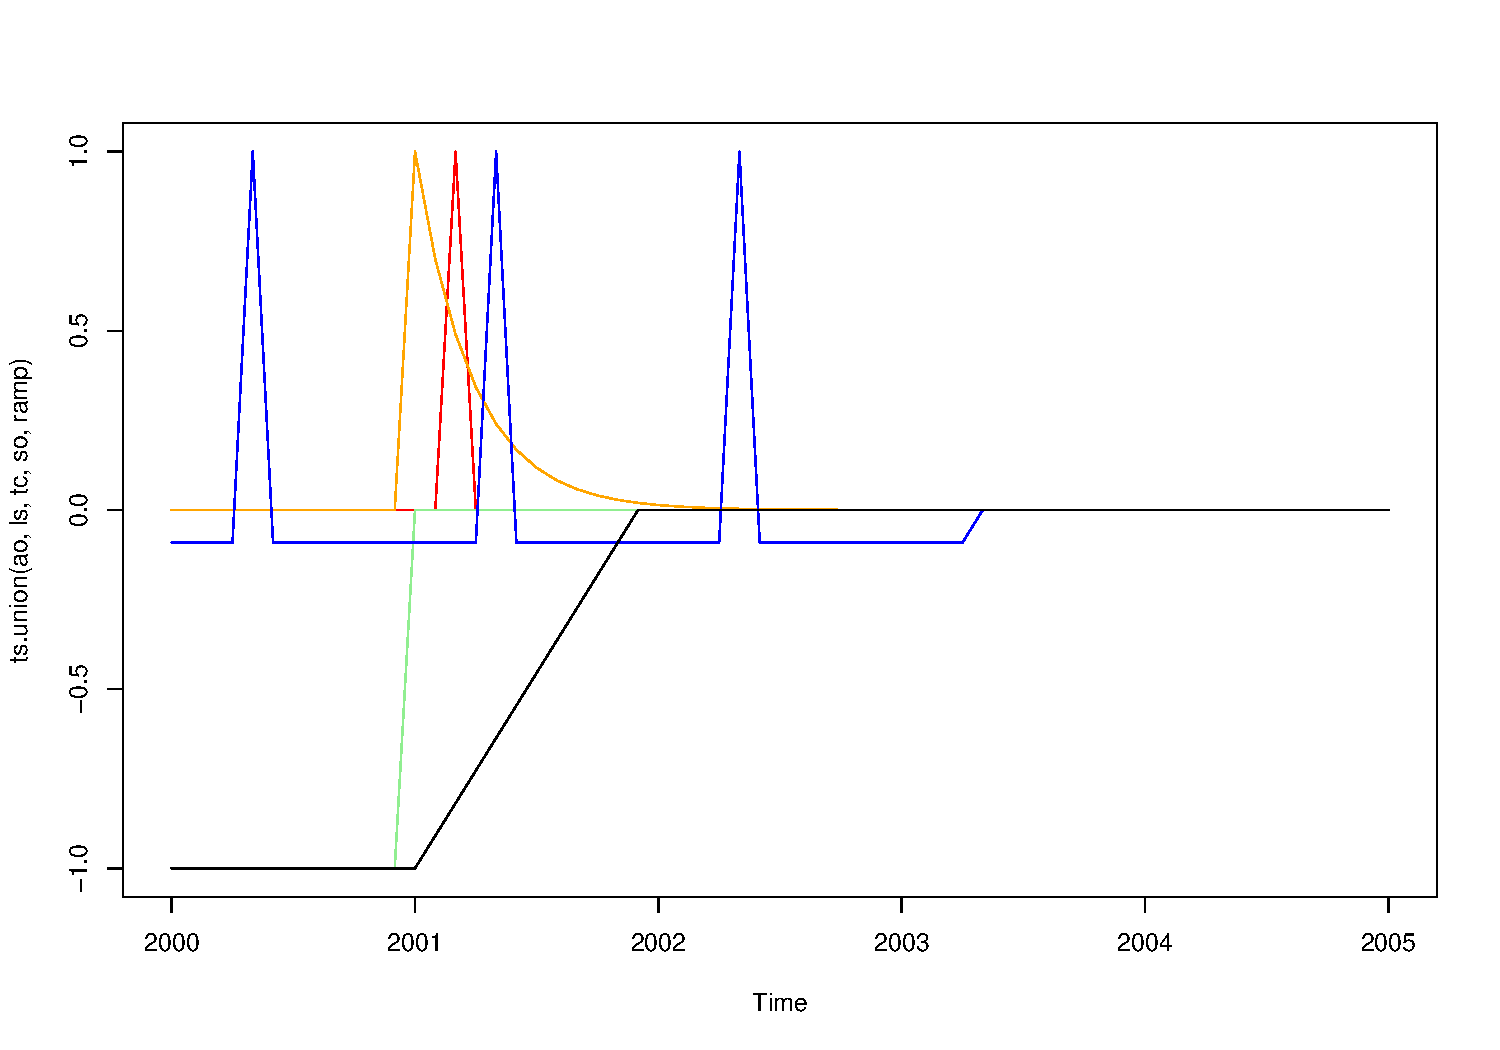
\includegraphics{img/markdown-outplot-1} \end{center}
\end{frame}

\hypertarget{time-series-tools}{%
\section{Time series tools}\label{time-series-tools}}

\begin{frame}[fragile]{Time series tools: NEW features in version 3}
\protect\hypertarget{time-series-tools-new-features-in-version-3}{}
The spirit of version 3 is to offer more tools from JDemetra+ libraries
such as:

\begin{itemize}
\item
  tests (seasonality, normality, randomness, residual trading
  dayseffects) in rjd3tookit, rjd3modelling and rjd3sa packages
\item
  autocorrelation functions (in rjd3toolkit), incl partial and inverse
\item
  arima model estimation and decomposition (rjd3modelling)
\item
  aggregation to higher frequency (\texttt{rjd3toolkit::aggregate()})
\end{itemize}

More flexibility for the user as they can be applied any time not just
as part of an SA processing.

Some of might also be available in other R packages. Arima model
estimation is notoriously faster than other R functions.
\end{frame}

\begin{frame}[fragile]{Testing for seasonality}
\protect\hypertarget{testing-for-seasonality}{}
In rjd3sa:

\begin{itemize}
\item
  Canova-Hansen (\texttt{seasonality.canovahansen()}) spctral, allows
  identifying patterns in HF data
\item
  X-12 combined test (\texttt{seasonality.combined()})
\item
  F-test on seasonal dummies (\texttt{seasonality.f()})
\item
  Friedman Seasonality Test (\texttt{seasonality.friedman()})
\item
  Kruskall-Wallis Seasonality Test
  (\texttt{seasonality.kruskalwallis()})
\item
  Periodogram Seasonality Test (\texttt{seasonality.periodogram()})
\item
  QS Seasonality Test (\texttt{seasonality.qs()})
\end{itemize}
\end{frame}

\begin{frame}[fragile]{Arima estimation}
\protect\hypertarget{arima-estimation}{}
\footnotesize

\begin{Shaded}
\begin{Highlighting}[]
\CommentTok{\# JD+}
\FunctionTok{print}\NormalTok{(}\FunctionTok{system.time}\NormalTok{(}
    \ControlFlowTok{for}\NormalTok{ (i }\ControlFlowTok{in} \DecValTok{1}\SpecialCharTok{:}\DecValTok{1000}\NormalTok{) \{  }
\NormalTok{      j }\OtherTok{\textless{}{-}}\NormalTok{ rjd3modelling}\SpecialCharTok{::}\FunctionTok{sarima.estimate}\NormalTok{(}
        \AttributeTok{data =} \FunctionTok{log}\NormalTok{(rjd3toolkit}\SpecialCharTok{::}\NormalTok{ABS}\SpecialCharTok{$}\NormalTok{X0.}\DecValTok{2}\NormalTok{.}\DecValTok{09}\NormalTok{.}\FloatTok{10.}\NormalTok{M), }
        \AttributeTok{order =} \FunctionTok{c}\NormalTok{(}\DecValTok{2}\NormalTok{, }\DecValTok{1}\NormalTok{, }\DecValTok{1}\NormalTok{), }\AttributeTok{seasonal =} \FunctionTok{list}\NormalTok{(}\AttributeTok{order =} \FunctionTok{c}\NormalTok{(}\DecValTok{0}\NormalTok{, }\DecValTok{1}\NormalTok{, }\DecValTok{1}\NormalTok{), }\AttributeTok{period =} \DecValTok{12}\NormalTok{))}
\NormalTok{    \}))}
\CommentTok{\#       user    system        elapsed (in seconds) }
\CommentTok{\#      4.98        0.37        4.63 }

\CommentTok{\#R{-}native}
\FunctionTok{print}\NormalTok{(}\FunctionTok{system.time}\NormalTok{(}
  \ControlFlowTok{for}\NormalTok{ (i }\ControlFlowTok{in} \DecValTok{1}\SpecialCharTok{:}\DecValTok{1000}\NormalTok{) \{  }
\NormalTok{    r }\OtherTok{\textless{}{-}} \FunctionTok{arima}\NormalTok{(}
      \AttributeTok{x =} \FunctionTok{log}\NormalTok{(rjd3toolkit}\SpecialCharTok{::}\NormalTok{ABS}\SpecialCharTok{$}\NormalTok{X0.}\DecValTok{2}\NormalTok{.}\DecValTok{09}\NormalTok{.}\FloatTok{10.}\NormalTok{M), }
      \AttributeTok{order =} \FunctionTok{c}\NormalTok{(}\DecValTok{2}\NormalTok{, }\DecValTok{1}\NormalTok{, }\DecValTok{1}\NormalTok{), }\AttributeTok{seasonal =} \FunctionTok{list}\NormalTok{(}\AttributeTok{order =} \FunctionTok{c}\NormalTok{(}\DecValTok{0}\NormalTok{, }\DecValTok{1}\NormalTok{, }\DecValTok{1}\NormalTok{), }\AttributeTok{period =} \DecValTok{12}\NormalTok{))}
\NormalTok{  \}))}
\CommentTok{\#       user    system        elapsed (in seconds) }
\CommentTok{\#     158.74        0.23      160.49 }

\FunctionTok{print}\NormalTok{(j}\SpecialCharTok{$}\NormalTok{likelihood )}
\FunctionTok{print}\NormalTok{(r)}
\end{Highlighting}
\end{Shaded}
\end{frame}

\hypertarget{conclusion}{%
\section{Conclusion}\label{conclusion}}

\begin{frame}[fragile]{SA in R: What's new in v3 ?}
\protect\hypertarget{sa-in-r-whats-new-in-v3}{}
Tests and time series tools

General and flexible defintion of

\begin{verbatim}
- calendars

- auxilary variables
\end{verbatim}

Refresh Policies

Direct setting of basic benchmarking
\end{frame}

\end{document}
